%TODO synthèse
%TODO glossaire et bibliographie etc ..

%%%%%%%%%%%%%%%%%%%%%%%%%%%%%%%%%%%%%%%%%%%%%%%%%%%%%%%%%
%                      Préambule                        %
%%%%%%%%%%%%%%%%%%%%%%%%%%%%%%%%%%%%%%%%%%%%%%%%%%%%%%%%%

%%%%%%%%%%%%%%%%%%%%%%%%%%%%%%%%%%%%%%%%%%%%%%%%%%%%%%%%%%%%%%%%%
%                      Préambule type                          %
%%%%%%%%%%%%%%%%%%%%%%%%%%%%%%%%%%%%%%%%%%%%%%%%%%%%%%%%%%%%%%%%



\def\changemargin#1#2{\list{}{\rightmargin#2\leftmargin#1}\item[]}
\let\endchangemargin=\endlist 

%%%%%%%%%%%%%%%%%% Classe dudit Document %%%%%%%%%%%%%%%%%%%%%%%
\documentclass[a4paper,12pt,openany]{report} % sert à définir des propriétés e base sur les articles
% Autre paramètres connnus: 	*book => pour de vrais livres
%				*article pour des artiles dans des revues scientifiques, des présentations, des rapports courts, des documentations, des invitation etc....
%				*report por des rapports plus long contenant plusieurs chapitres, des petits livres, des thèses
%				*Slides pour des transparants
%				*foiltex
% Option: Xpt taille de la police,  4apaper/letterpaper/a5paper/b5paper/executivepaper, fleqn, leqno, titlepage/notitlepage indique si une nouvelle page doit être commencée après le titre du document, twocolumn,twoside/oneside,



%%%%%%%%%%%%%%%%%%%%%%%% Package %%%%%%%%%%%%%%%%%%%%%%%%%%%%%%%
\usepackage{doc}% permet de documenter des programmes (cf doc.dtx]
\usepackage{exscale} % fournit des version de taille de caractère que LaTeX va utiliser (cf ltexscale.dtx)
\usepackage{fontenc} % spécifie le codage des police de caractère que LaTeX va utiliser (cf ltoutenc.dtx)
%\usepackage[latin]{inputenc} %Autorise les caractères acentués
\usepackage{ifthen} % fournit des commandes de conditions (cf ifthen.dtx)
\usepackage{latexsym} %permet l'utilisation de la police des symboles LaTeX
\usepackage{makeidx} %fournit des commandes pour réaliser un index
\usepackage{syntonly} % analyse le doc sans le formater
\usepackage[T1]{fontenc}
\usepackage[utf8x]{inputenc} 
%\usepackage[utf8]{inputenc}% permet de spécifier le codeage des caractère utiliser dans le source.
\usepackage[english,francais]{babel}
%\usepackage{asmath} %Fonctions servant à l'écriture mathématique
\usepackage{xspace} %Fonctions permettant d'introduire des espaces
\usepackage{xargs} %Permet d'utiliser de définir plus simplement des fonctions
\usepackage{trace}%Permet d'utiliser des traces de debbug
\usepackage{show2e}% debbug
\usepackage[pdftex]{graphicx}
\usepackage{hyperref}

%%%%%%%%%%%%%%%%% Style du pied de page %%%%%%%%%%%%%%%%%%%%%%%%

\pagestyle{plain}% imprime le numéro de page au milieu du pied de page
%\pagestyle{heading}%imprime le titre du chapitre courant et le numéro dans l'en tête et laisse le pied de page vide.
%\pagestyle{empty}% laisse l'en tête et le pied de page vide


%Nota bene: On peut changer le pied de page en court en utilisant \thispagestyle


%%%%%%%%%%%%%%%%% Césure   %%%%%%%%%%%%%%%%%%%%%%%%

\hyphenation{FORTRAN}
\hyphenation{An-ti-cons-ti-tu-tion-nel-le-ment}

%%%%%%%%%%%%%%%% Citation Environement %%%%%%%%%%%%

\newsavebox{\nomepigraphe}
\newenvironment{epigraphe}[1]
	{% clause begin
	\vspace*{-1.5cm}%
	\small\sffamily% mise en évidence
	\savebox{\nomepigraphe}{#1}% une boîte pour sauvegarder
	% l’ origine de la citation
	\slshape% tout est penché
	\begin{changemargin}{0pt}{-2cm}% on se met au large
	\begin{flushright}}% tout est poussé à droite
	{% clause end
	\\[4pt]\usebox{\nomepigraphe}.% insertion de l’origine
	\end{flushright}%
	\end{changemargin}\par\vspace*{0.6cm}}

%
\input ./preambule.tex %sans saut de ligne


%%%%%%%%%%%%%%Titre%%%%%%%%%%%%%%%%%%%%%%%%%%%%%%%%%%%%
\title{ Projet de 3 année à l'INSA Centre Val de Loire } % Titre du document
\author{BAIZ Mamoune && BAIZ Mamoune} % Auteur
\date{\today} % Date de création


%%%%%%%%%%%%%%%%%%%%%%%Debut Doc%%%%%%%%%%%%%%%%%%%%%%%
\begin{document} % Début du document
%%%%%%%%%%%%%%%%%%%%%%Page de Garde%%%%%%%%%%%%%%%%%%%%
{
\begin{titlepage}
  \begin{sffamily}
  \begin{center}

    % Upper part of the page. The '~' is needed because \\
    % only works if a paragraph has started.
    
\includegraphics[scale=0.5]{Images/png/insa_logo.png}~\\[1.5cm]

    \textsc{\LARGE Institut National des Sciences Appliquées  Centre Val de Loire }\\[2cm]

    \textsc{\Large Rapport de projet 3\up{ème} année option 2SU}\\[1.5cm]

    % Title
%    \HRule 
%	\\[0.4cm]
    { \huge \bfseries Domotique\\[0.4cm] }

%    \HRule 
%	\\[2cm]
    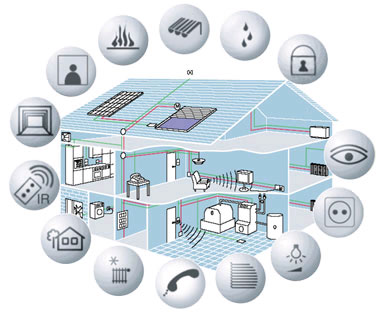
\includegraphics[scale=0.5]{Images/jpg/domotic.jpg}
    \\[2cm]

    % Author and supervisor
    \begin{minipage}{0.4\textwidth}
      \begin{flushleft} \large
        BAIZ Mamoune et MUNIER Marc \\
        Promo 2016\\
      \end{flushleft}
    \end{minipage}
    \begin{minipage}{0.4\textwidth}
      \begin{flushright} \large
        \emph{Encadrant :} M. Briffaut\\
      \end{flushright}
    \end{minipage}

    \vfill

    % Bottom of the page
    {\large 9 Février 2016}

  \end{center}
  \end{sffamily}
\end{titlepage}
}
%%%%%%%%%%%%%%%%%%%%%%%Page Vierge%%%%%%%%%%%%%%%%%%%%
\newpage
\newpage



%%%%%%%%%%%%%%%%%%%%% Remerciment %%%%%%%%%%%%%%%%%%%%
\newpage
\section*{Remerciement}
Au terme de notre formation à L’INSA Centre Val de Loire, et tout au long de ce projet il est nécessaire de remercier tous mes professeurs, ainsi que tout le corps professoral et administratif de notre établissement, auxquels je tiens à rendre hommage pour leurs efforts prodigieux qu’ils n’ont cessé de fournir afin que nous puissions, mes collèges et moi, avoir une formation solide et rigoureuse ; pour leur encadrement tout au long de cette année, et pour leur disponibilité permanente. Je n’oublierais pas de remercier spécialement M.Briffaut pour son soutien tout au long du projet, ainsi que ces précieux cours de "domotique" qui nous ont aidés à réaliser ce projet.\newline

%marc: ok pour moi peut etre revoir la forme
\clearpage
\newpage
%%%%%%%%%%%%%%%%%%%%%Résumé%%%%%%%%%%%%%%%%%%%%%%%%%%%
\section*{Résumé}
\vspace{20pt} 
\label{chap-savoir}
\begin{epigraphe}{Les proverbes Pr \textbf{21} 11}
Quand on châtie le railleur, le simple s’assagit ;\\
quand on instruit le sage, celui-ci gagne en savoir.
\end{epigraphe}

   Votre résumé commence ici...
   ...

\newpage
%%%%%%%%%%%%%%%%%%%%%table des matières%%%%%%%%%%%%%%%
\tableofcontents
\clearpage

%%%%%%%%%%%PLAN
%
%\section*{Introduction} %( comment on a fait ce projet, en quoi il consiste, les enjeux )
%Mamoune
%Mamoune: Dans cette partie il est conseillé de prendre une photo représentant la conception 
%		C)	l'application
% 
%III)	Comment le mettre en place Marc
%V)		Nos difficulté
%VII)	Conclusion
%
%V)		Nos diffficultés difficulté
%VII)	Conclusion (fini)
%
%Ne pas oublier l'annexe
%Ne pas oublier le glossaire.
%
% chaque partie est à ecrire dans un fichier indépandant du main
% il suffit de rajouter la ligne suivante pour inclure ces écrits
%\input ./maPartie.tex %sans saut de ligne
%
%%%%%%%%%%%%%%%%%%%


%%%%%%%%%%%%%%%%%%%%%%%%%%%%%%%%%%%%%%%%%%%%%%%%%%%%%%

\newpage
\chapter{Introduction}

Ce projet se présente comme une très bonne expérience sur le plan théorique et pratique, car il permet de concevoir une première approche sur le monde des objets connectés et plus spécialement en domotiques. Il constitue aussi une occasion unique pour mettre en évidence le cumul des connaissances que nous avons acquis tout au long de notre formation spécialisée en sécurité ubiquitaire.


De ce fait, notre binôme a décidé de réaliser un projet concernant la domotique. Toutefois, il est nécessaire de définir ce qu'est la domotique. La domotique est l'ensemble des techniques de l'électronique, de physique du bâtiment, d'automatisme, de l'informatique et des télécommunications utilisées dans les bâtiments, plus ou moins « interopérables » et permettant de centraliser le contrôle des différents systèmes et sous-systèmes de la maison et de l'entreprise (chauffage, volets roulants, porte de garage, 
portail d'entrée, prises électriques, etc.). La domotique vise à apporter des solutions techniques pour répondre aux besoins de 
confort (gestion d'énergie, optimisation de l'éclairage et du chauffage), de sécurité (alarme) et de communication (commandes à 
distance, signaux visuels ou sonores, etc.) que l'on peut retrouver dans les maisons, les hôtels, les lieux publics, etc.


Ce projet consiste alors à créer une petite centrale domotique grâce à une raspberry, permettant d'informer l'utilisateur sur certaines données reçues par des capteurs. Cette mini centrale permettera alors à l'utilisateur d'améliorer son confort et surtout sa sécurité. Ceci ne pourrait être que bénéfique envers les utilisateurs potentiels. La domotique est de plus en plus présente dans notre quotidien. Grâce à elle nous pouvons alors économiser de l'énergie ( gestion du chauffage, gestion de l'éclairage, gestion des volets ), augmenter l'autonomie des personnes handicapées ( assistance à l'ouverture des portes, des fenêtres, des volets, pilotage des appareils électriques, commande vocale ) ou encore améliorer la sécurité de nos habitations ( système d'alarme ). La mise en place d'un système domotisé peut se faire dès la construction d'un bâtiment ( norme KNX ), lors d'une rénovation, ou encore de façon ponctuelle ( norme X10 ).




%%%%%%%%%%%%%%%%%%%%%%%%part II %%%%%%%%%%%%%%%%%%%%%%

\newpage
\chapter{Presentation du projet}
\section{les outils} 
Afin de réaliser ce projet, quelques outils et éléments nous ont été indispensables. Tout d'abord, la centrale qui contrôle tout le système de domotique: La Raspberry Pi.

Le Raspberry Pi est un nano-ordinateur monocarte à processeur ARM conçu par le créateur de jeux vidéo David Braben, dans le cadre de sa fondation Raspberry Pi. Cet ordinateur, qui a la taille d'une carte de crédit, est destiné à encourager l'apprentissage de la programmation informatique. Il permet l'exécution de plusieurs variantes du système d'exploitation libre GNU/Linux et des logiciels compatibles à plusieurs protocole de domotique. Il est fourni nu (carte mère seule, sans boîtier, alimentation, clavier, souris ni écran) dans l'objectif de diminuer les coûts et de permettre l'utilisation de matériel de récupération.
Cet outil est alors la pièce maîtresse de notre projet domotique. 
\subsection{Description de la raspberry pi 2}
%TODO inclure photo raspberry pi 2
\begin{description}
	\item[Environnement] \hfill \\ Linux (Debian, Fedora et ArchLinux), RISC OS , Windows IOT
	\item[Système d'exploitation] \hfill \\ Linux (Raspbian, Pidora, et Arch Linux ARM gentoo), RISC OS, FreeBSD, NetBSD, Windows 10 IoT (uniquement compatible avec le Raspberry Pi 2), Plan 9
	\item[Alimentation] \hfill \\ Micro-USB 5 V
	\item[Processeur] \hfill \\
		\begin{itemize}
			\item Broadcom BCM2835 - ARM1176JZF-S 700 MHz (modèle 1) ou 1 GHz (Modèle Zero)1
			\item Broadcom BCM2836 - Cortex-A7 900 MHz (modèle 2)
		\end{itemize}

	\item[Stockage] \hfill \\ Carte SD (A, B), Carte microSD (A+,B+,2)
	\item[Mémoire] 
		\begin{itemize}
			\item 256 Mo (modèle A et A+)
			\item 256 Mo (modèle B rev 1)
			\item 512 Mo (modèle B rev 2 et B+)
			\item 1 Go (modèle 2)
		\end{itemize}

	\item[Carte graphique] \hfill \\ Broadcom VideoCore IV1,
	\item[Connectivité] \hfill \\ USB, Ethernet (modèle B, B+ ,2) (RJ45), HDMI, RCA, Jack 3,5 mm, Micro USB
	\item[Dimensions] \hfill \\ 
		\begin{itemize}
			\item 85,60 mm × 53,98 mm × 17 mm (A, B, B+),
			\item 65 mm × 53,98 mm × 17 mm (A+),
			\item 65 mm × 30 mm × 5 mm (Zero)
		\end{itemize}
	\item[Poid] \hfill \\ 44,885 g (A, B, B+), 23 g (A+)
\end{description}

\subsection{Les composants utilisés}
Afin de savoir les données concernant le milieu ambiant contournant la centrale de domotique (la raspberry pi2), il est nécessaire d'utiliser des capteurs pour capturer les données que nous souhaitons, mais aussi d'une antenne posée sur la raspberry analysant les données qu'elle reçoit depuis les capteurs.

\subsubsection{Antenne}
Nous avons utilisée une antenne Z-Wave. Z-Wave est un protocol radio conçu pour la domotique, facilement intégrée avec la raspberry pi2. Z-Wave fonctionne dans la gamme de fréquences sous-gigahertz, qui dépend des régions (868 MHz en Europe, 908 MHz aux US, et d'autres fréquences suivant les bandes ISM des régions). La portée est d'environ 50 m (davantage en extérieur, moins en intérieur). La technologie utilise la technologie du maillage (mesh) pour augmenter la portée et la fiabilité.

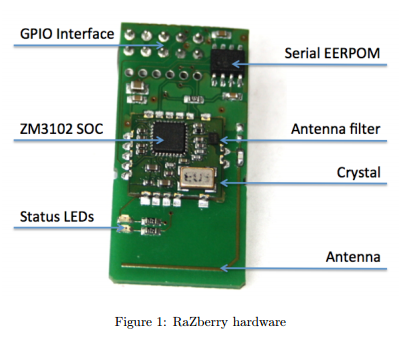
\includegraphics[scale=0.5]{./latex/Images/png/Zwave.png}\newline

Etant donné que le protocole Z-Wave se base sur une seule plage de fréquence il est donc vulnérable à un brouilleur de fréquence.
 De plus le protocole lui-même semble souffrir de problèmes de sécurité.Dans l'état actuel de cette norme, il semble plus prudent de ne confier à Z-Wave que des tâches domotiques limitées aux éléments dont le dysfonctionnement ou le piratage ne pose pas de problème.
\subsubsection{Capteurs}

\begin{description}
\item[FIBARO Smoke Sensor] \hfill \\

\end{description}
Ce détecteur est très sensible à la fumée, mais pas juste à la fumée. Certains matériaux brûlent avant de capter la fumée sous haute température.
Voilà pourquoi les ingénieurs de  FIBARO ont décidé d'inclure une protection supplémentaire: un capteur de fumée sous la forme d'un capteur de température.
 Si la quantité de fumée n'est pas assez suffisante pour déclencher l'alarme, l'appareil sera toujours en mesure de détecter la menace.
En effet il est sensible à un changement rapide de température provoqué par un feu. Il détecte aussi lorsque la température dépasse les 54°C. Ceci est alors suffisant pour le capteur de fumée pour découvrir la menace et signaler les utilisateurs à ce sujet. 

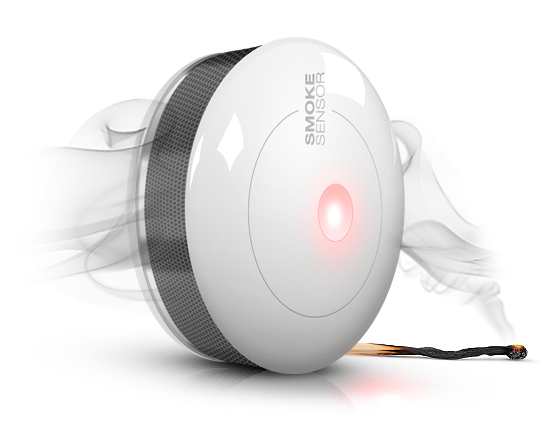
\includegraphics[scale=0.5]{./latex/Images/smoke.png}\newline


FIBARO Flood Sensor:

Le capteur d'innondation FIBARO , une taille compacte et une grande variété de fonctions supplémentaires . Ce capteur est tout simplement remarquable ! Ce dispositif unique peut vous garantir une sécurité optimale . Avec sa technologie de pointe et de précision , le capteur d'innondation Fibaro vous alerte de crue menaçante , ou un changement radical de température . Tout en étant sans entretien et sans la nécessité d'une installation professionnelle .


\includegraphics[scale=0.5]{./latex/Images/png/Fibaro.png}\newline
LA FIBARO Wall Plug, une prise murale, qui permet d'indiquer, la consommation de la puissance électrique qui passe en courant, en temps réel sous forme d'un halo lumineux autour de la prise.

Ce capteur respecte des normes de sécurité très exigeantes, et obligatoires dans certains pays nordiques.


-Protection enfants et fonction veilleuse.


-Configuration ultra-simple grâce à l'unique bouton est aux indications lumineuses.


-Puissance maximale autorisée :

    *2500W (11A) avec charge résistive (éclairage incandescent / halogène, radiateur, four à convection, etc.).
    

    *1500W (8A) avec charge capacitive (ampoules LED ou Fluo, TV et appareils électroniques, four MO, plaques à indiction,etc.).
    
    
    *En cas de doute sur le type de charge, ne dépassez pas 1500W.


-Fonction répéteur pour étendre le réseau Z-Wave.


-Modèle avec prise Française (Type E)


-Garantie 2 ans 
\subsection{le Logiciel domoticz}
Domoticz est un logiciel libre de gestion de domotique qui a pour but d’être exécutable sur un grand nombre de machines différente. Et ce qui fait son principal atout, c’est que le Raspberry Pi fait partie des machines sur lesquelles il peut tourner ! Ce qui permet donc d’en faire une machine dédiée aux opérations domotiques à prix très réduit. 

\subsection*{L'application}
Afin d'améliorer notre projet, nous avons décidé de réaliser une application android, permettant aux clients distants de pouvoir se connecter à distance pour accéder aux données partagées par la centrale domotique. Ainsi il pourra gérer son domicile, et créer des scénarios après certaines conditions. Dans la page d'accueil de l'application, l'utilisateur devrait choisir une des chambres ou domiciles qui possédent afin qu'il puisse découvrir l'état de ce dernier. Il a aussi la possibilité d'en rajouter une nouvelle chambre, ou domicile pour qu'il arrive à faire les modifications souhaitées.\newline
Néanmoins, faute de temps, nous avons pas pu aboutir au résultat souhaité, l'application affiche une page générique par défaut pour toutes les chambres. Cette application n'était pas un élément crucial de notre projet, mais elle aurait pu améliorer notre projet considérablement. Cette thématique pourra alors ouvrir la possibilité de générer de nouveaux projets, essayant de répondre à ce besoin.\newline
Le code source de cette application sera mis en annexe.\newline
Nous avons aussi utilisé, l'interface web proposée par Z-WaveMe afin de générer des scénarios en respectant des conditions (If ---> Then). Avec cet outil, nous avons pu générer plusieurs scénarios. Des vidéos de démonstration se trouvent dans ces liens.\newline
% Liens de vidéos youtube de démo si possible
Dans l'interface Web proposée par Z-waveMe, un fichier de log existe permettant à l'utilisateur de pouvoir visualiser tout ce qui se passe pendant la journée concernant les capteurs.


%Une photo de raspberry pi2 doit être mise ici TODO
%%%%%%%%%%%%%%%%%%%%%%%%partie III%%%%%%%%%%%%%%%%%%%%

%\input ./III_MiseEnPlace.tex %sans saut de ligne

%%%%%%%%%%%%%%%%%%%%%%%%%%%%%%%%%%%%%%%%%%%%%%%%%%%%%%%
\newpage
\chapter{Les problèmes rencontrées}
Tout au long du projet, nous avons rencontré quelques difficultés, que nous avons réussi à résoudre. Dans ce chapitre, nous allons décrire tous les problèmes rencontrés, et les solutions que nous avons décidé pour résoudre ces derniers.
\subsection{Cartes SD grillées }
Avant de commencer le projet, il nous ai été donné deux raspberry Pi et tous les composants qui va nous permettre de connecter la raspberry Pi2 et de s'en servir.\newline
Parmi ces éléments de raspberry Pi, des cartes SD nous ont été offertes pour réaliser le projet. Néanmoins, parmi plusieurs cartes SD, un grand nombre été non fonctionnelles, et d'autres ont cessé de fonctionner après certains essais avec la raspberry Pi2.\newline
A cause des installations nombreuses de système que nous avons dû réaliser tout au long du projet, nous avons décidé de travailler avec une seule raspberry Pi, et de changer la version de la raspberry Pi en raspberry Pi2, pour des raisons d'optimisation. Après cette manoeuvre, nous avons pu avancer plus rapidement, avec aucun souci de connexion ni de mémoire.
\subsection{Antenne Z-Wave}
Afin d'analyser les données des capteurs, une Antenne Z-Wave nous a été donnée. Cependant, parmi deux des Z-Wave données une ne marchait pas, ceci nous a encore poussé à éliminer une raspberry et de réaliser le projet avec une seule raspberry.
\subsection{Arrivée tardive du matériel (Antenne Z-Wave+Capteurs)}
Afin de faire le projet, un genre de matériel nous ai nécessaire, M.Briffaut nous alors commandé ce matériel pour réaliser ce projet. Toutefois, le matériel est arrivé un peu tardivement. Durant ce temps, nous nous sommes bien documentés pour mieux connaitre la domotique et ses enjeux, mais aussi, nous avons arrivé à bien installé le système sur nos raspberry respectives.   
%\subsection{ } % Je réaliserai cette partie c'est juste que je souhaite discuter avec toi à propos de cette partie 

\newpage
\chapter{Conclusion}
Dans cette époque le marché de la domotique est devenu un des projets les plus prometteurs, surtout avec la démocratisation des tablettes et smartphones, la fiabilité des technologies sans fil et l'émergence des objets connectés : toutes ces conditions affirment que la maison intelligente est un véritable marché de masse. Le nouveau paysage technologique permet en effet de proposer des solutions domotiques moins chères, plus évolutives et intuitives et surtout adaptées aux besoins des consommateurs (confort au sein du logement, économie d'énergie, sécurisation des biens, autonomie des personnes dépendantes, etc.).\newline

Durant le présent projet, il nous a été confié comme mission de réaliser une centrale domotique, réalisant des tâches visant à sécuriser la vie des utilisateurs et d'améliorer leurs confort. Nous étions alors dans l'obligation de mieux connaitre le monde de la domotique, afin que nous puissions mieux gérer le projet. Après une mûre connaissance, nous avons alors réussi à réaliser un projet en domotique permettant de gérer quelques capteurs et d'en créer des scénarios à l'issue de situations spécifiques.\newline

L'élaboration de ce travail nous a permis d'une part, d'approfondir nos connaissances acquises et le savoir faire que nous avons pu réaliser tout au long de cette année de spécialité 2SU, et d'autre part de découvrir les solutions que proposent le monde de la domotique.\newline

%%%%%%%%%%%  ANNEXE %%%%%%%%%%%%%%%%%%%
*Caractéristiques du capteur de fumée FIBARO:

 
Ce capteur répond à la nouvelle norme EN14604. -    Nouvelle version à la norme Norme EN14604


-    Fonction "boite noire" (mémoire des événements).


-    Sans-fil Z-Wave+.


-    Design et matériaux nobles.


-    Compact avec seulement 6,5x2,8cm


-    Sensibilité réglable.


-    Bouton de configuration et d'indication multicolore.


-    Alimentation par pile fournie 


-    Autonomie de 3 ans env. (peut varier suivant les paramètres de réveil et de transmission des températures).


-    Garantie 2 ans


-    Sans-fil Z-Wave+.

*Pour retrouver le code Android des différents programme Android réalisés, veuillez suivre ce lien:  \href{https://github.com/marcMunier/INSAdom/tree/master/InsaDomApp}


*Etapes pour la configuration et l'ajout d'un capteurs d'un capteur avec ZWaveMe:


-Ajout d'un capteur sur l'interface ZwaveMe:


--> Pour ajouter un élément, il faut tout d'abord appuyer sur la touche paramètre en haut à droite, et choisir Devices.
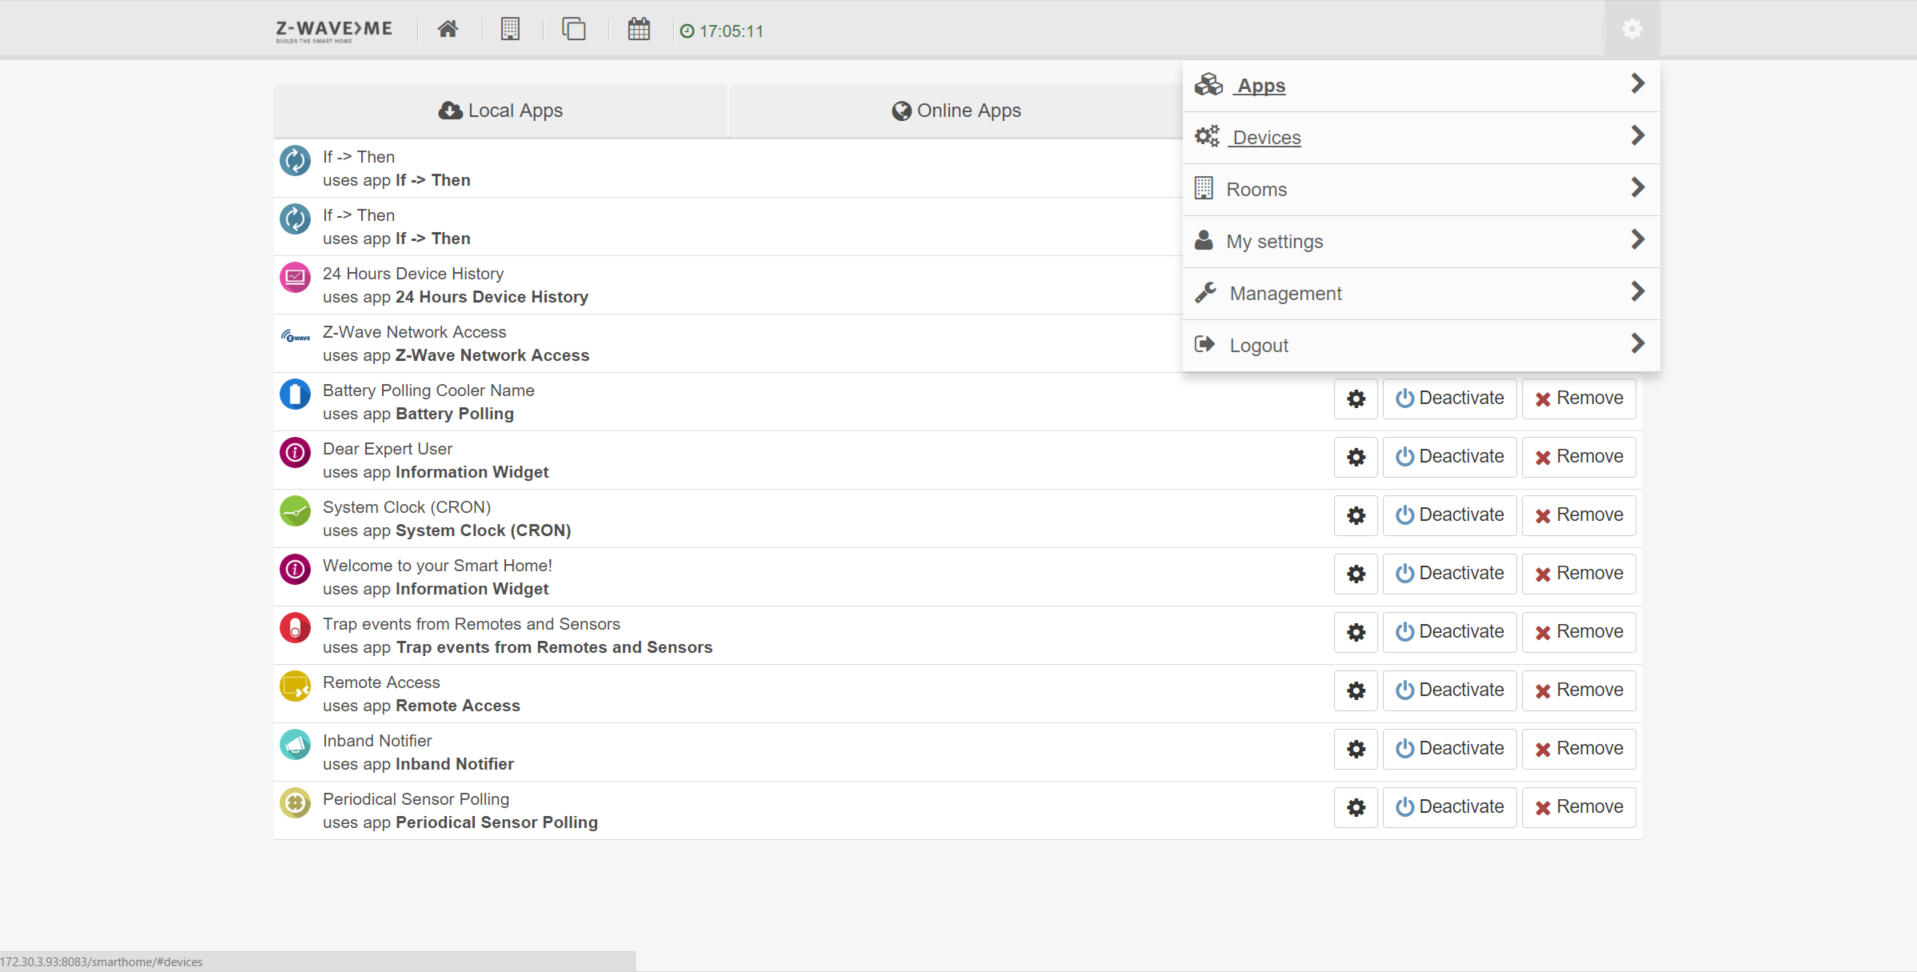
\includegraphics[scale=0.5]{./latex/Images/png/menu_zwaveme.png}\newline
 --> Appuyer dans la partie ZWave sur Add new
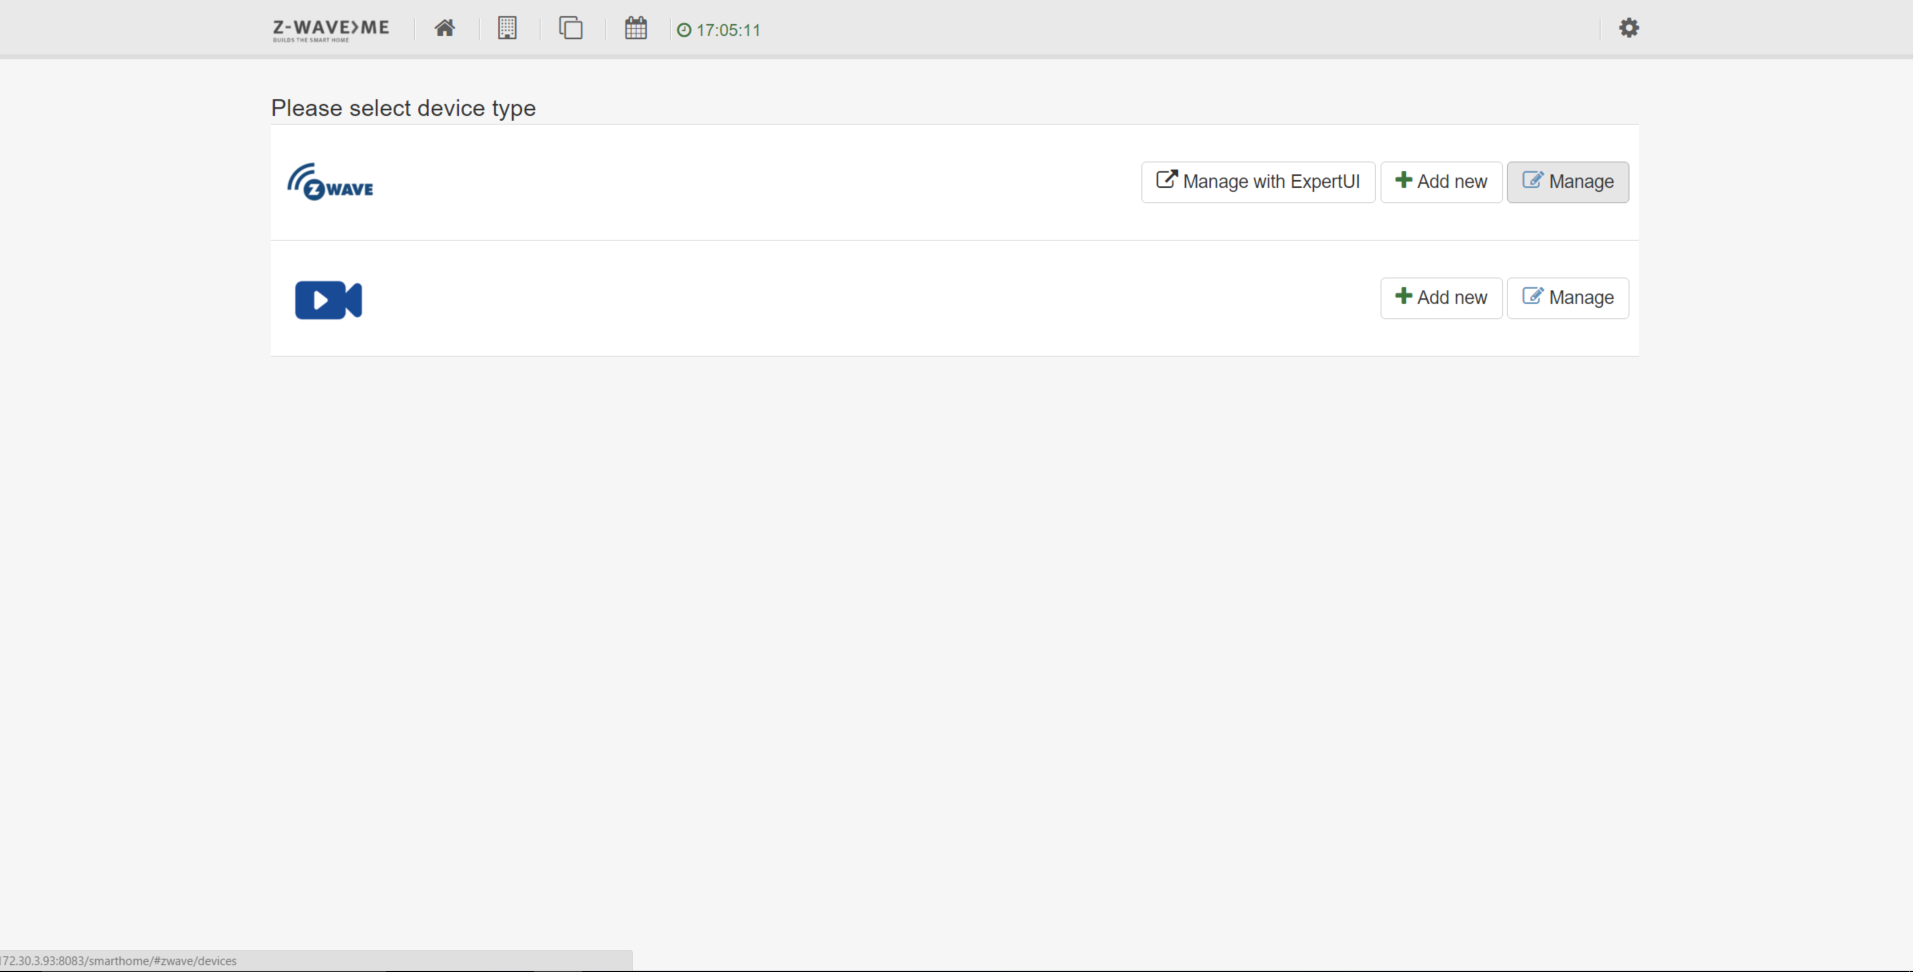
\includegraphics[scale=0.5]{./latex/Images/png/devices_zwaveme.png}\newline
--> Appuyer sur Start inclusion et réveiller votre matériel en suivant les règles de chaque capteur
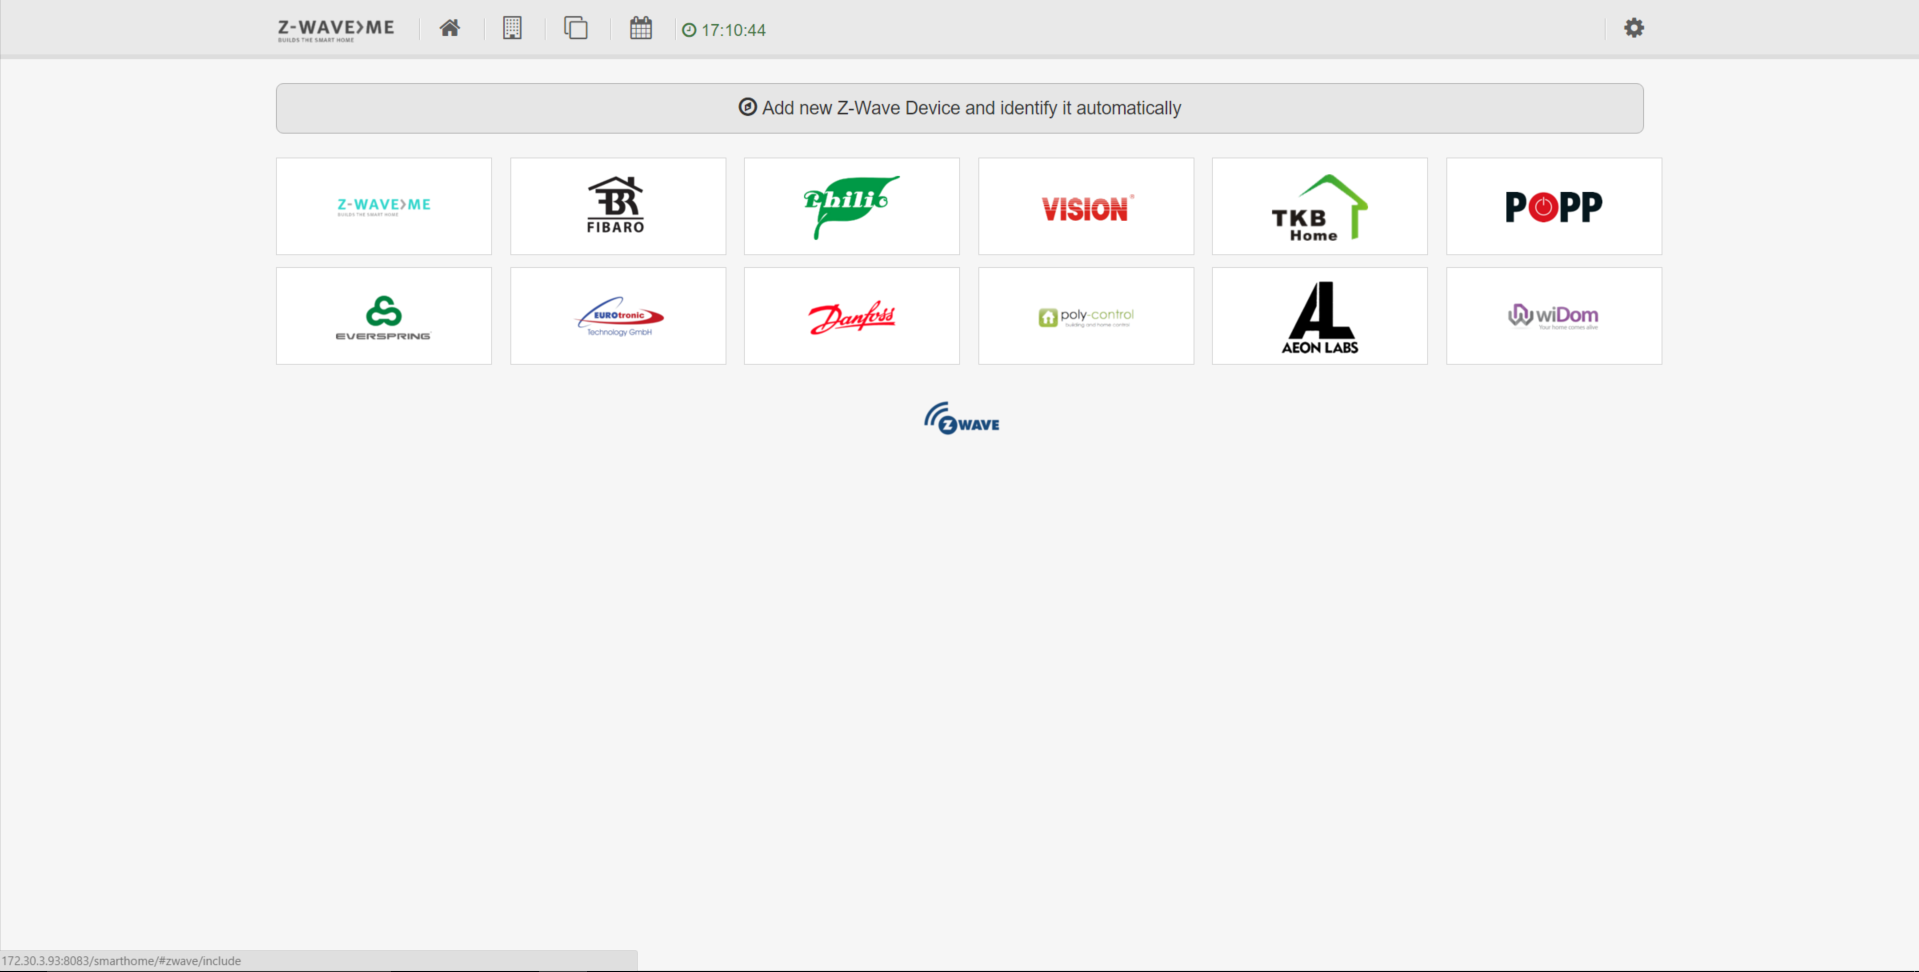
\includegraphics[scale=0.5]{./latex/Images/png/add_zwaveme.png}\newline
--> Laisser faire
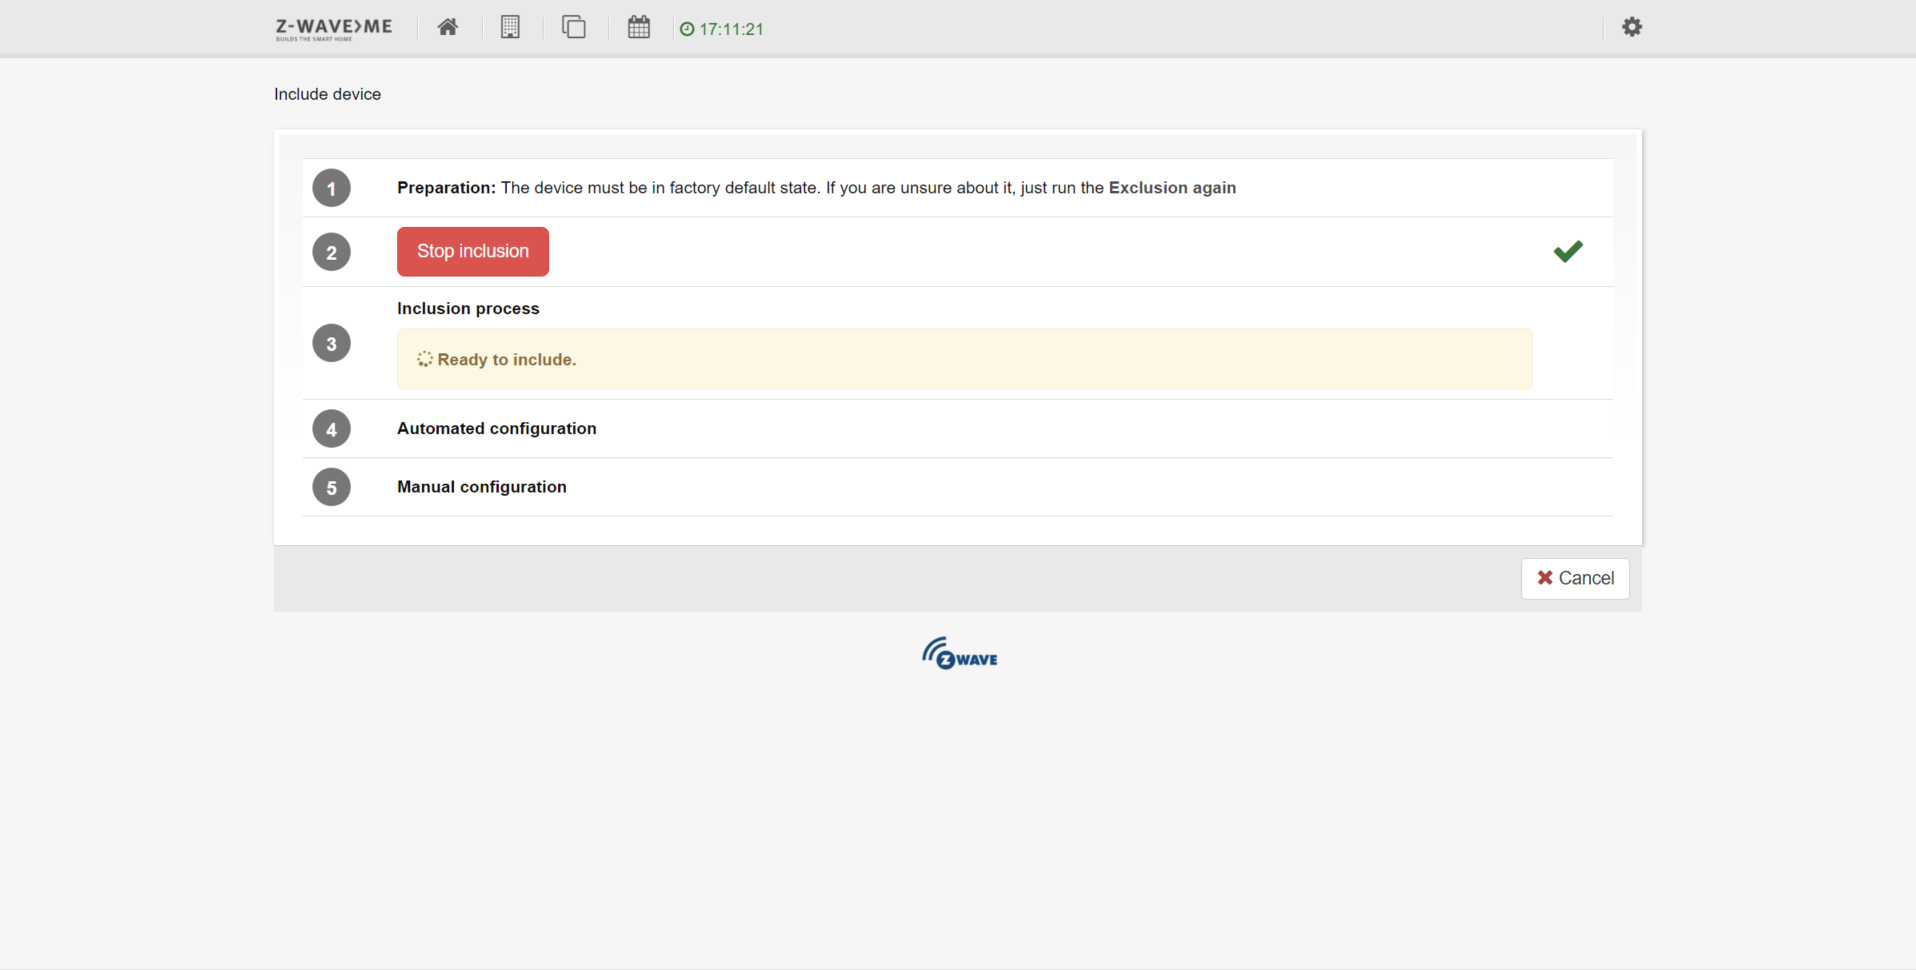
\includegraphics[scale=0.5]{./latex/Images/png/add2_zwaveme.png}\newline
--> L'élément est ajouté avec succès
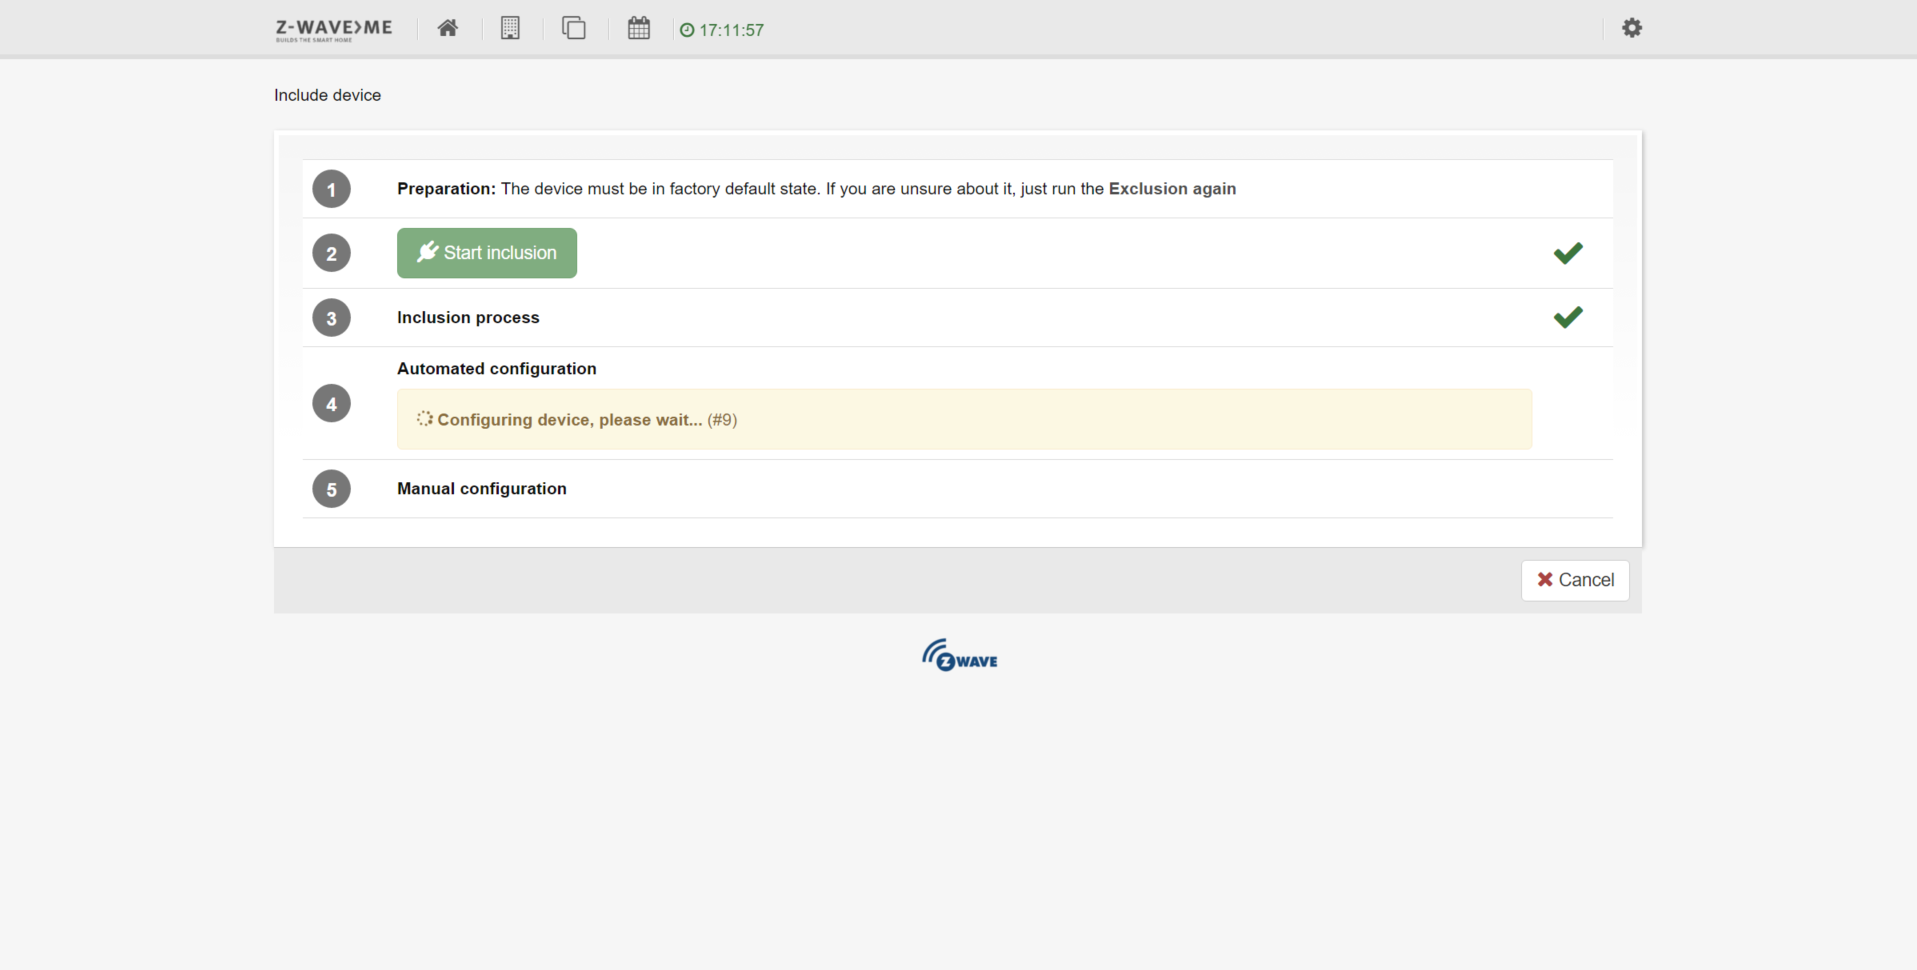
\includegraphics[scale=0.5]{./latex/Images/png/add3_zwaveme.png}\newline

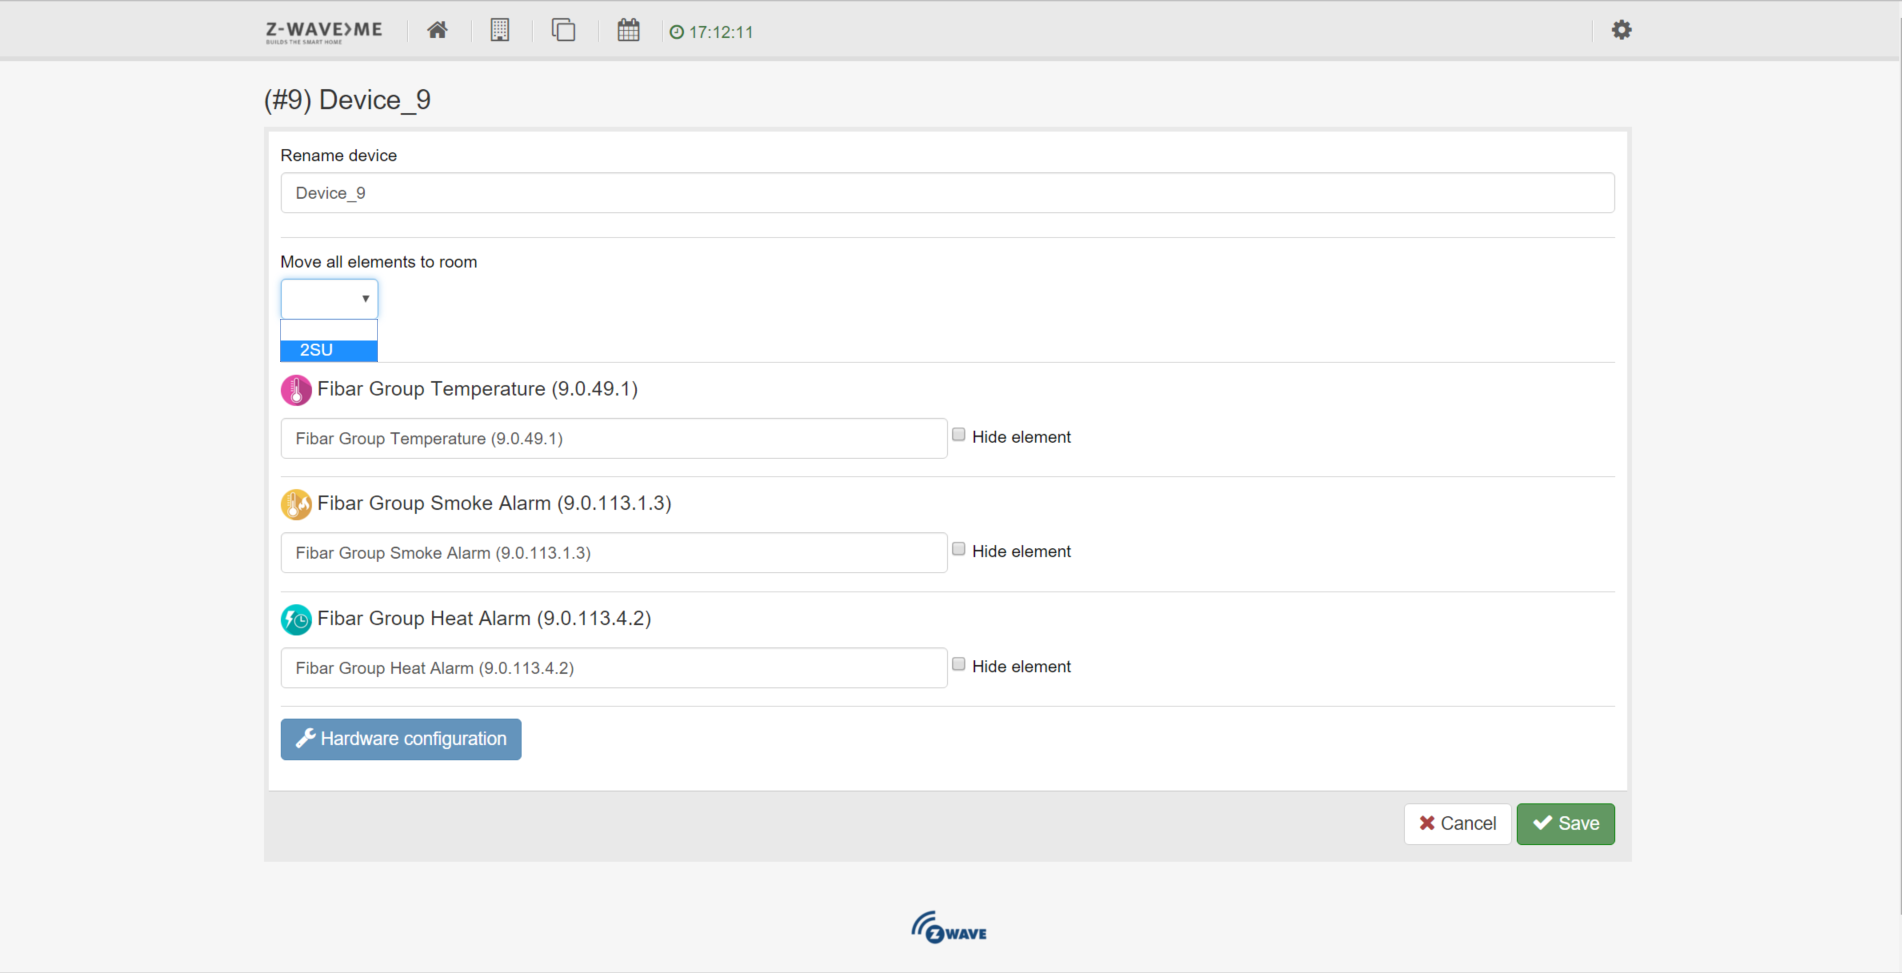
\includegraphics[scale=0.5]{./latex/Images/png/add4_zwaveme.png}\newline


-Les capteurs disponibles:

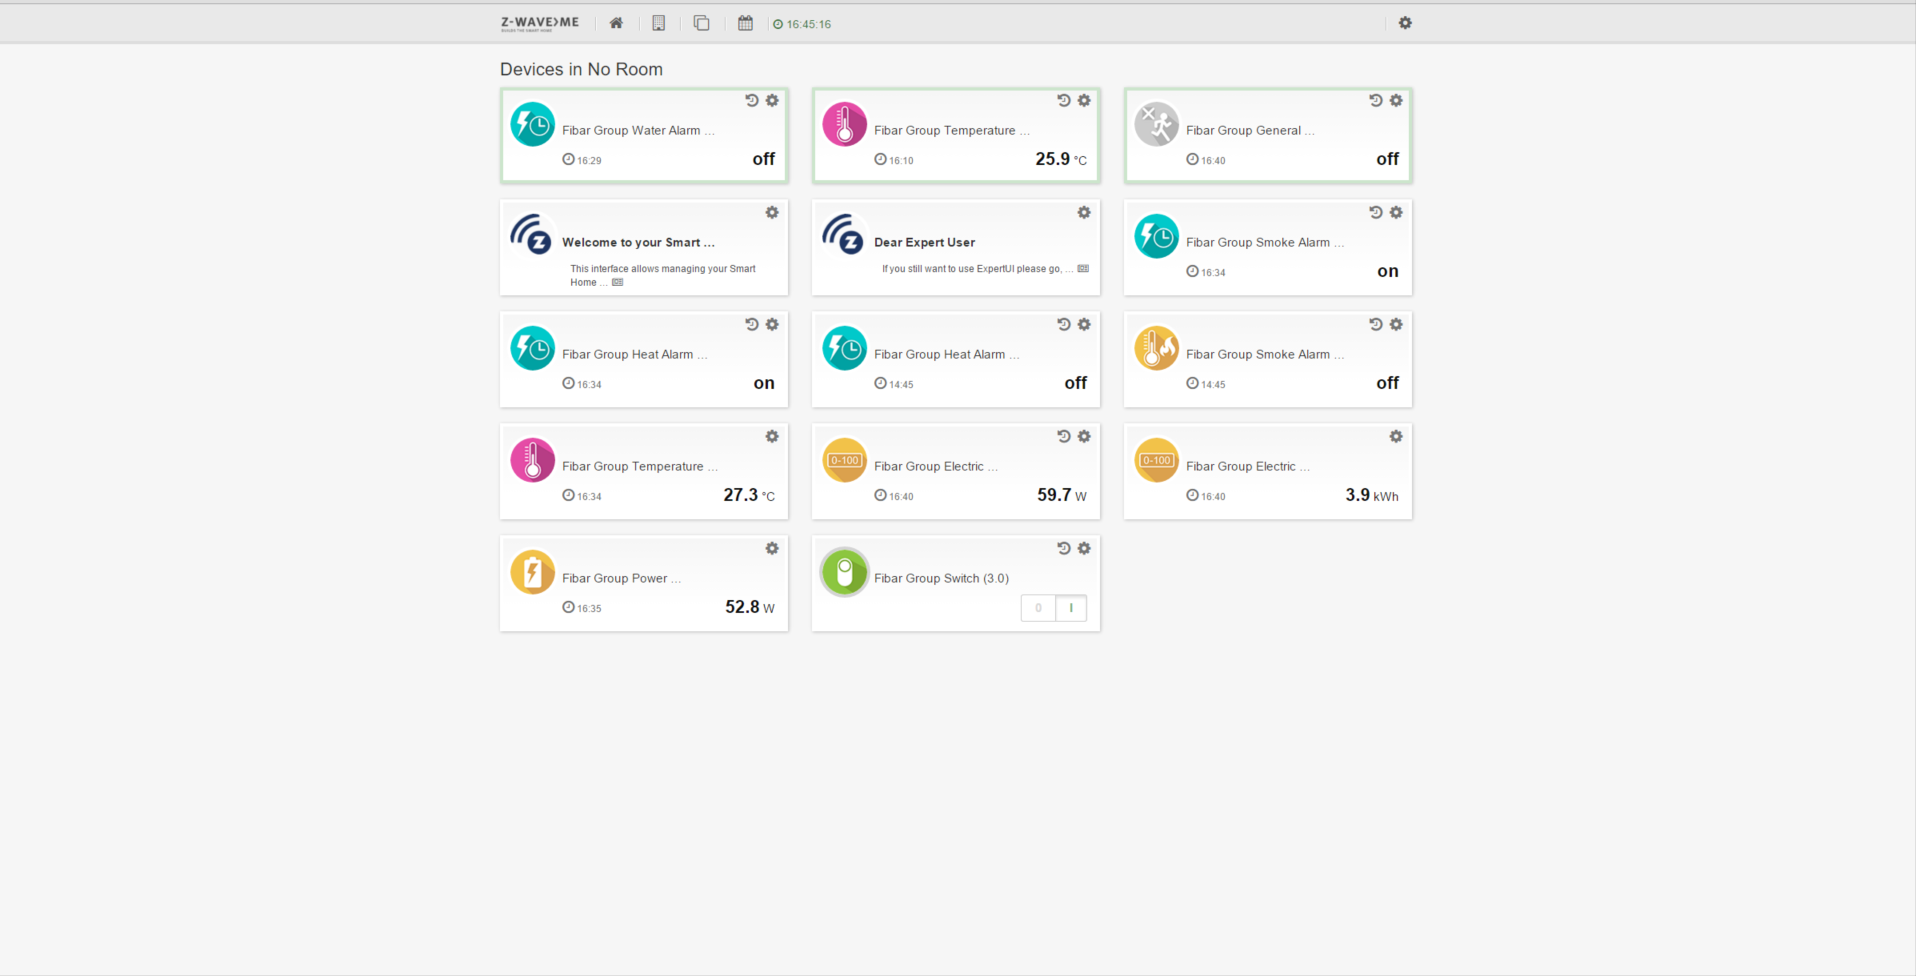
\includegraphics[scale=0.5]{./latex/Images/png/ecranCapteur.png}\newline

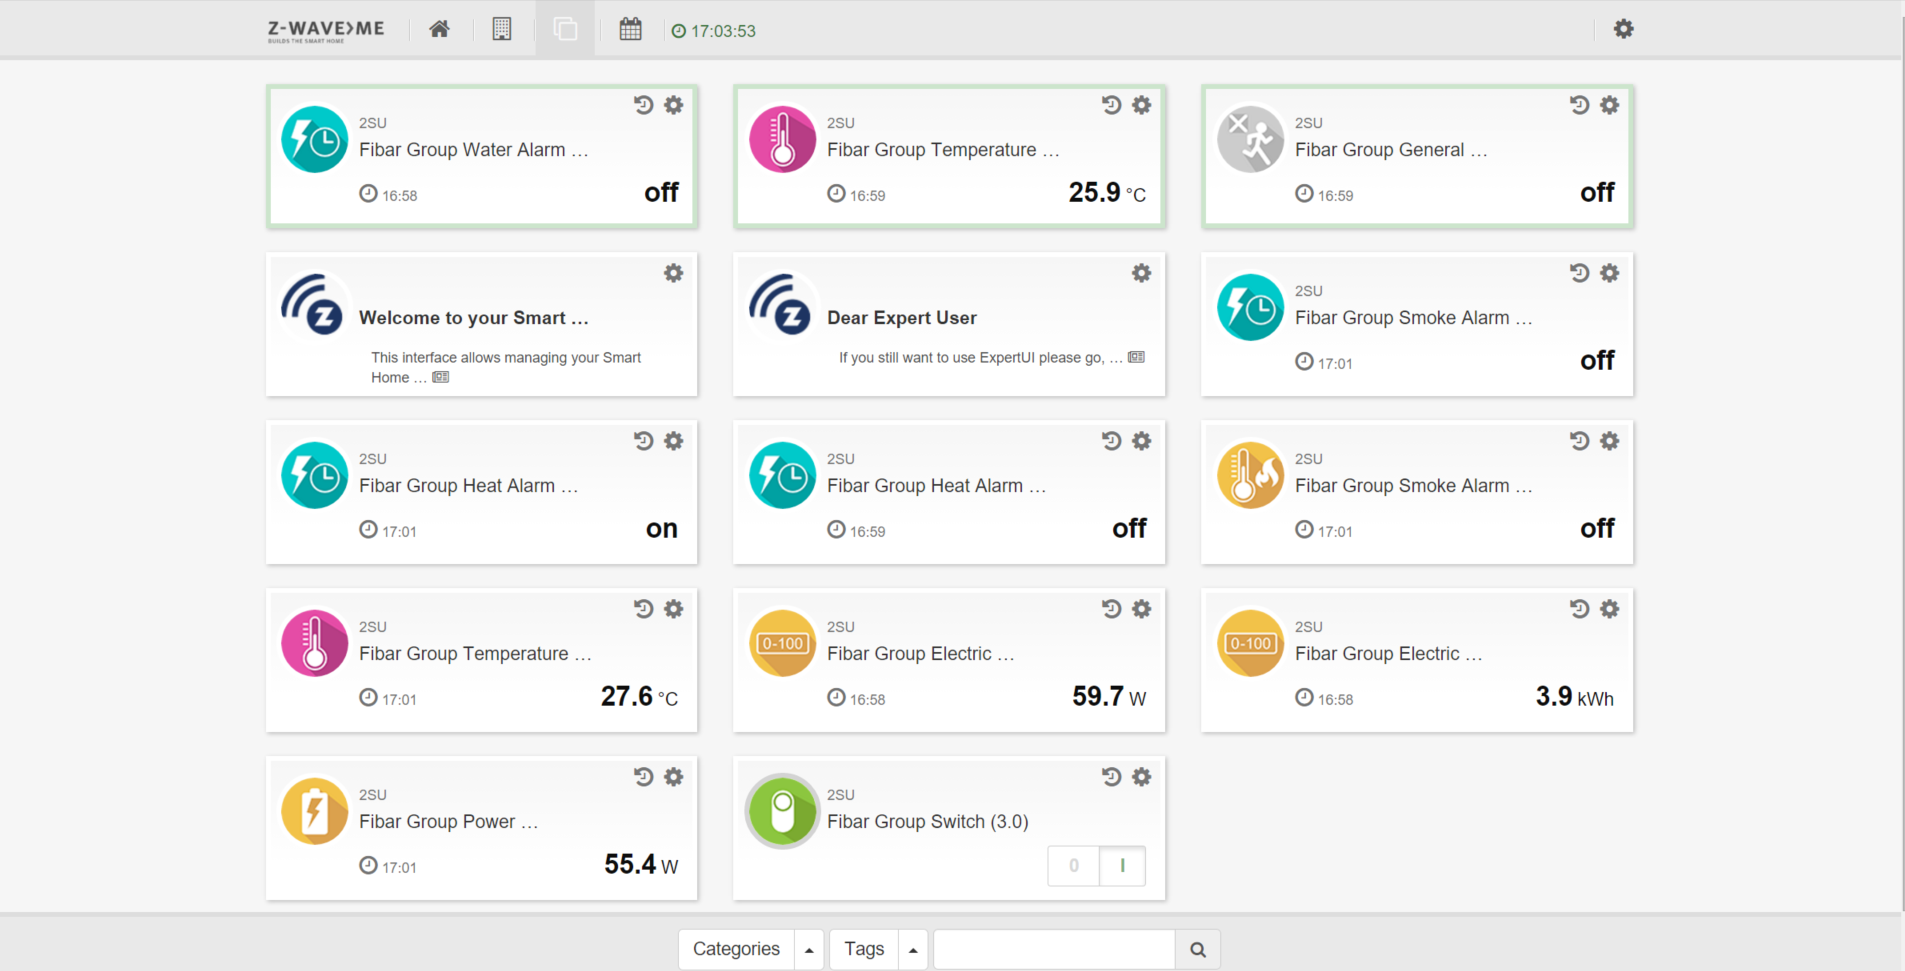
\includegraphics[scale=0.5]{./latex/Images/png/device_zwaveme.png}\newline


*Il existe deux modes de gestions des capteurs avec l'interface ZWaveMe, le mode home et le mode expert:


--> Le mode home
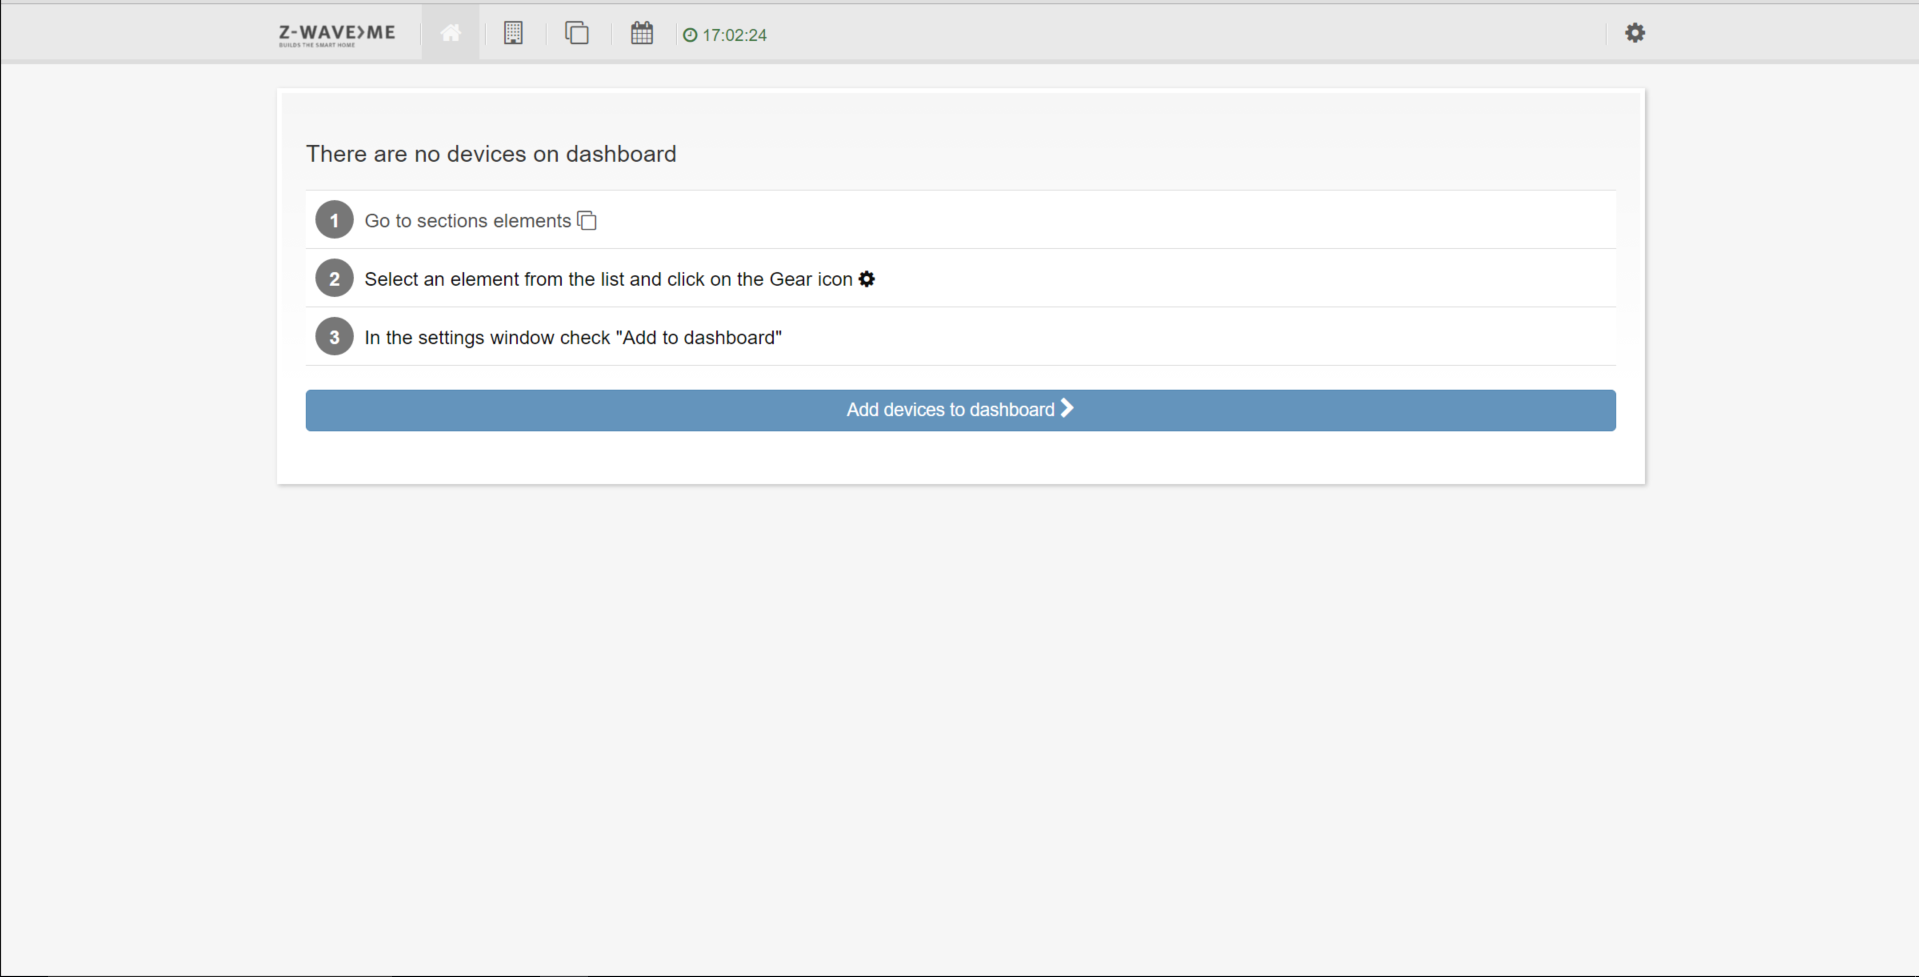
\includegraphics[scale=0.5]{./latex/Images/png/home_zwaveme.png}\newline

--> Pour accéder au mode expert il faut suivre le lien en haut de l'image

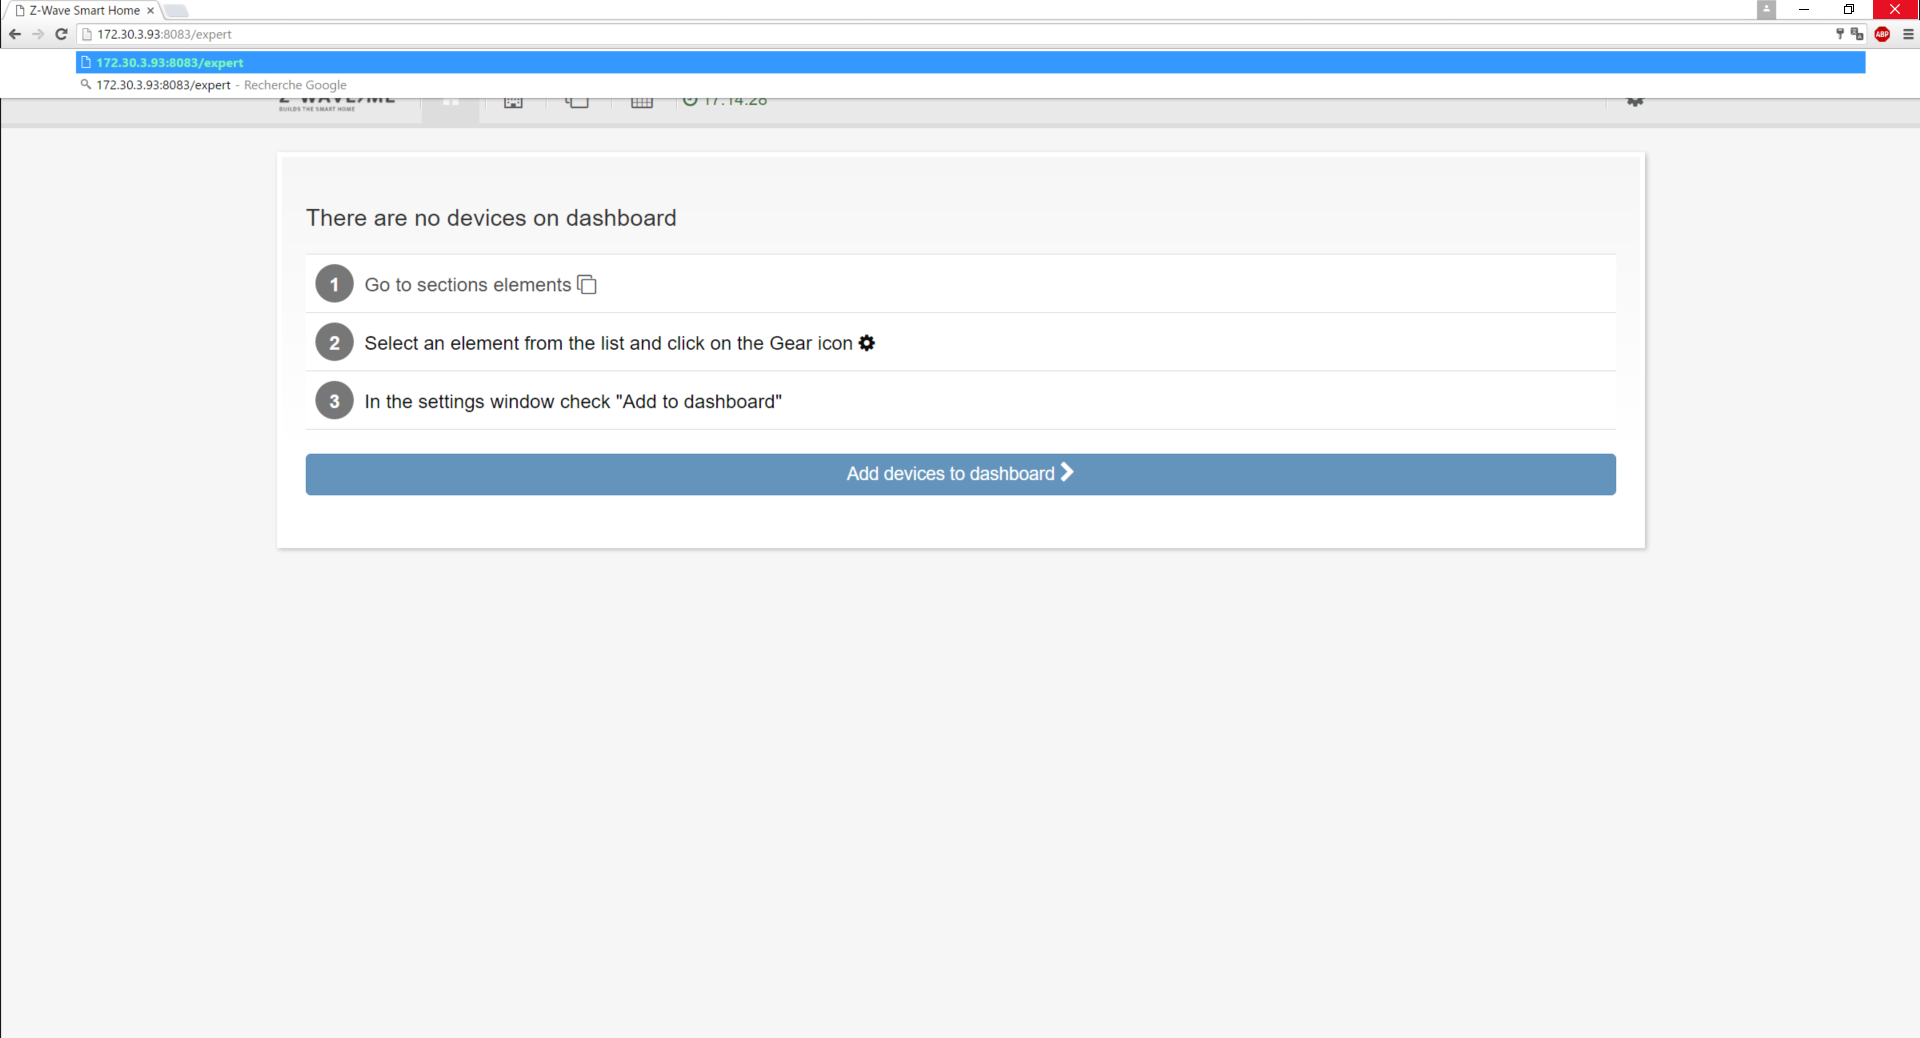
\includegraphics[scale=0.5]{./latex/Images/png/go_to_zwaveme.png}\newline

--> Mode expert

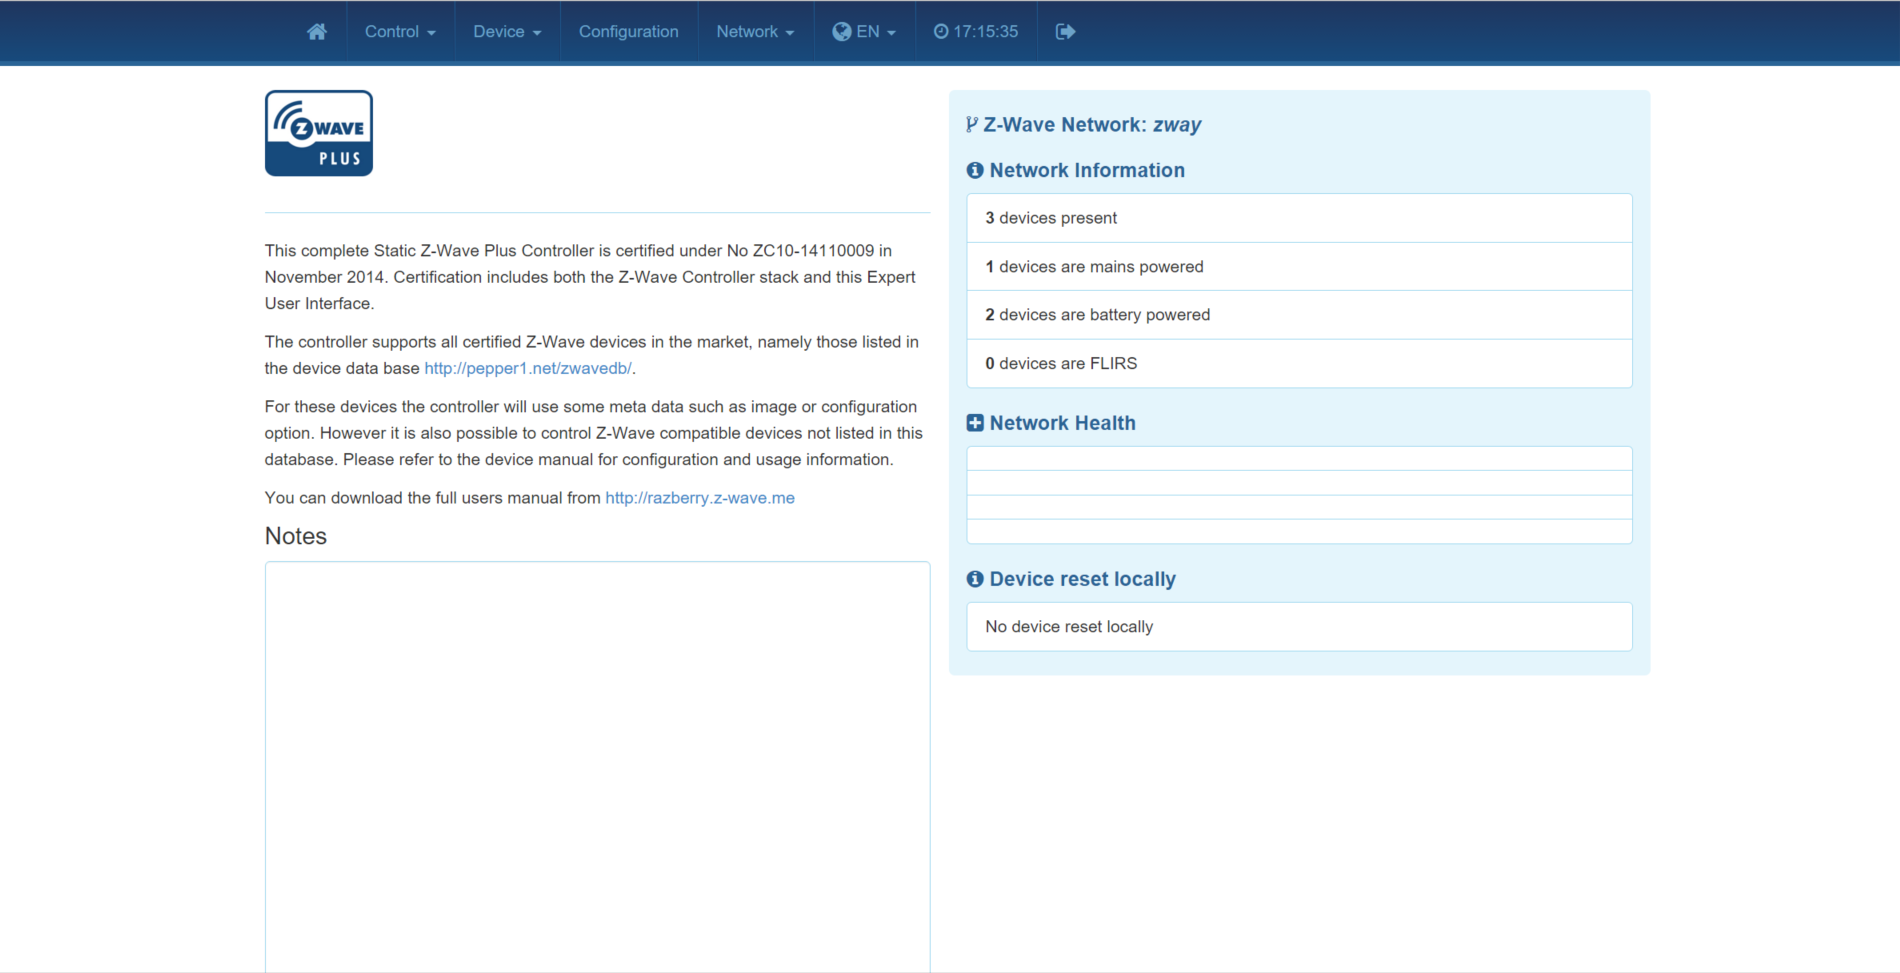
\includegraphics[scale=0.5]{./latex/Images/png/expert_zwaveme.png}\newline

* Pour gérer vos capteurs, l'interface Web ZWaveMe (mode home) propose une solution:

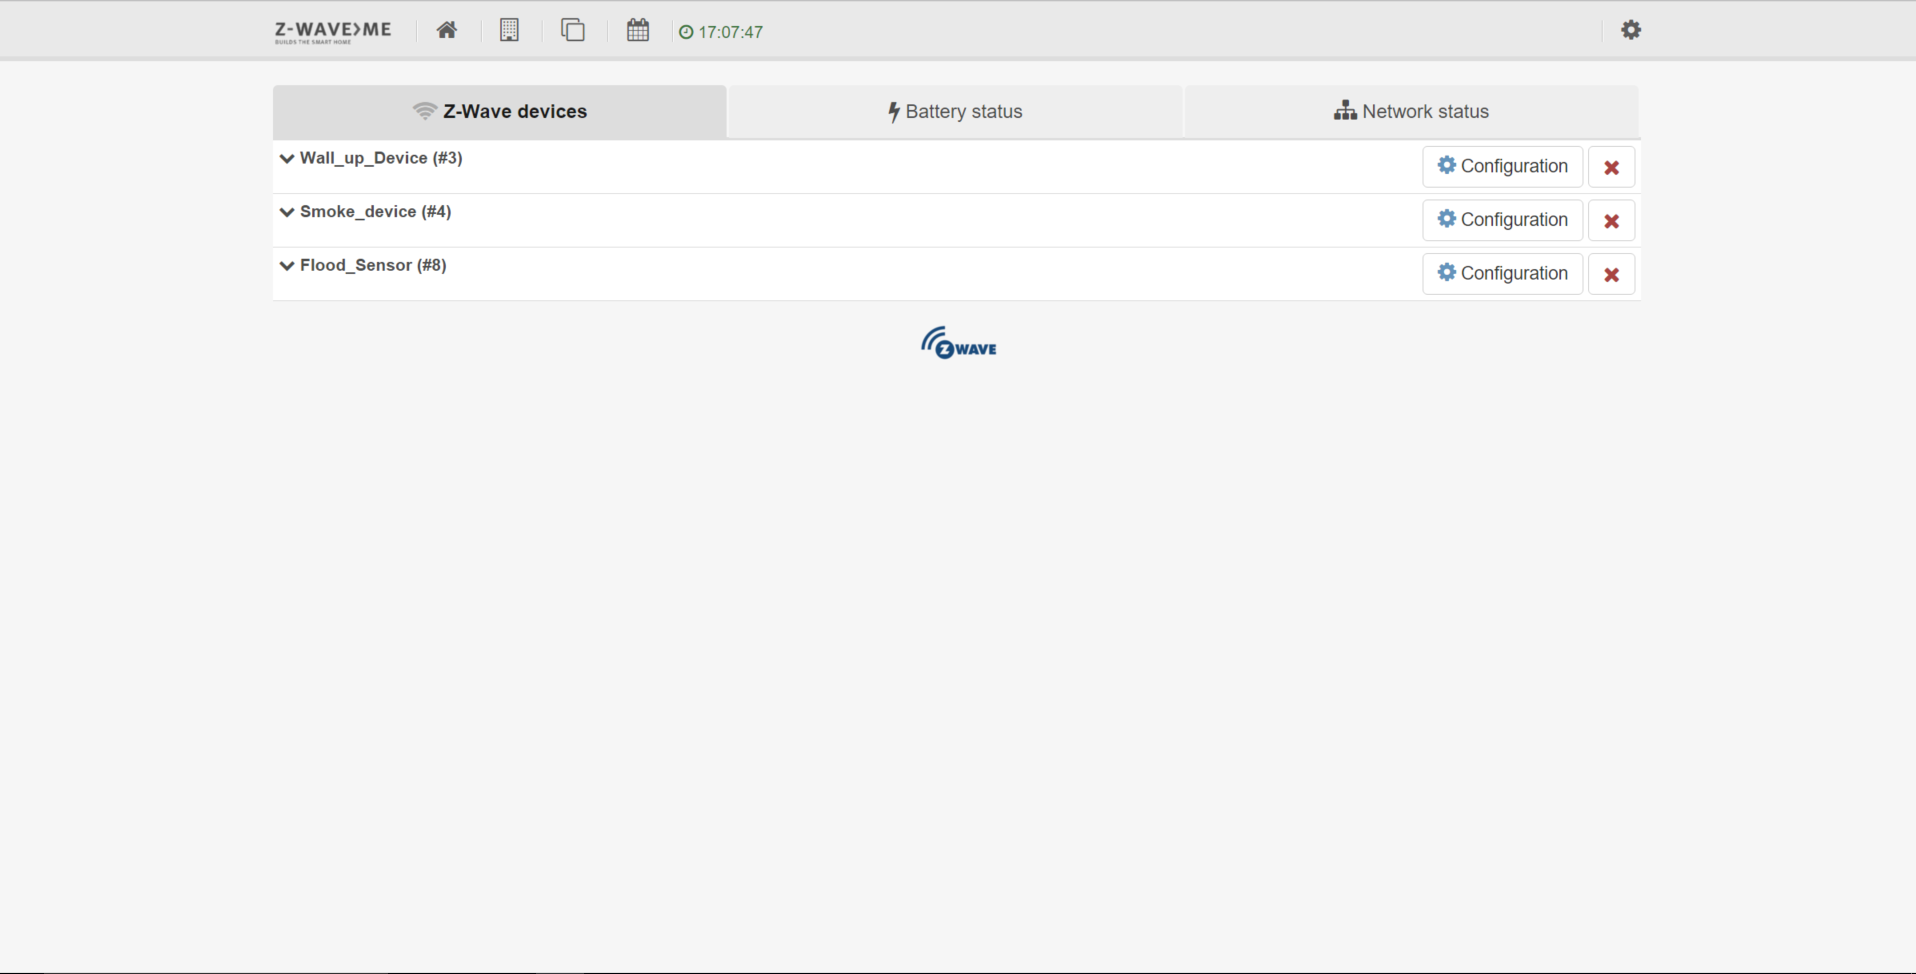
\includegraphics[scale=0.5]{./latex/Images/png/manage_zwaveme.png}\newline

* Si vous souhaitez supprimer un capteur (un device), vous avez la possibilité en suivant ces images:


--> Appuyer sur start exclusion


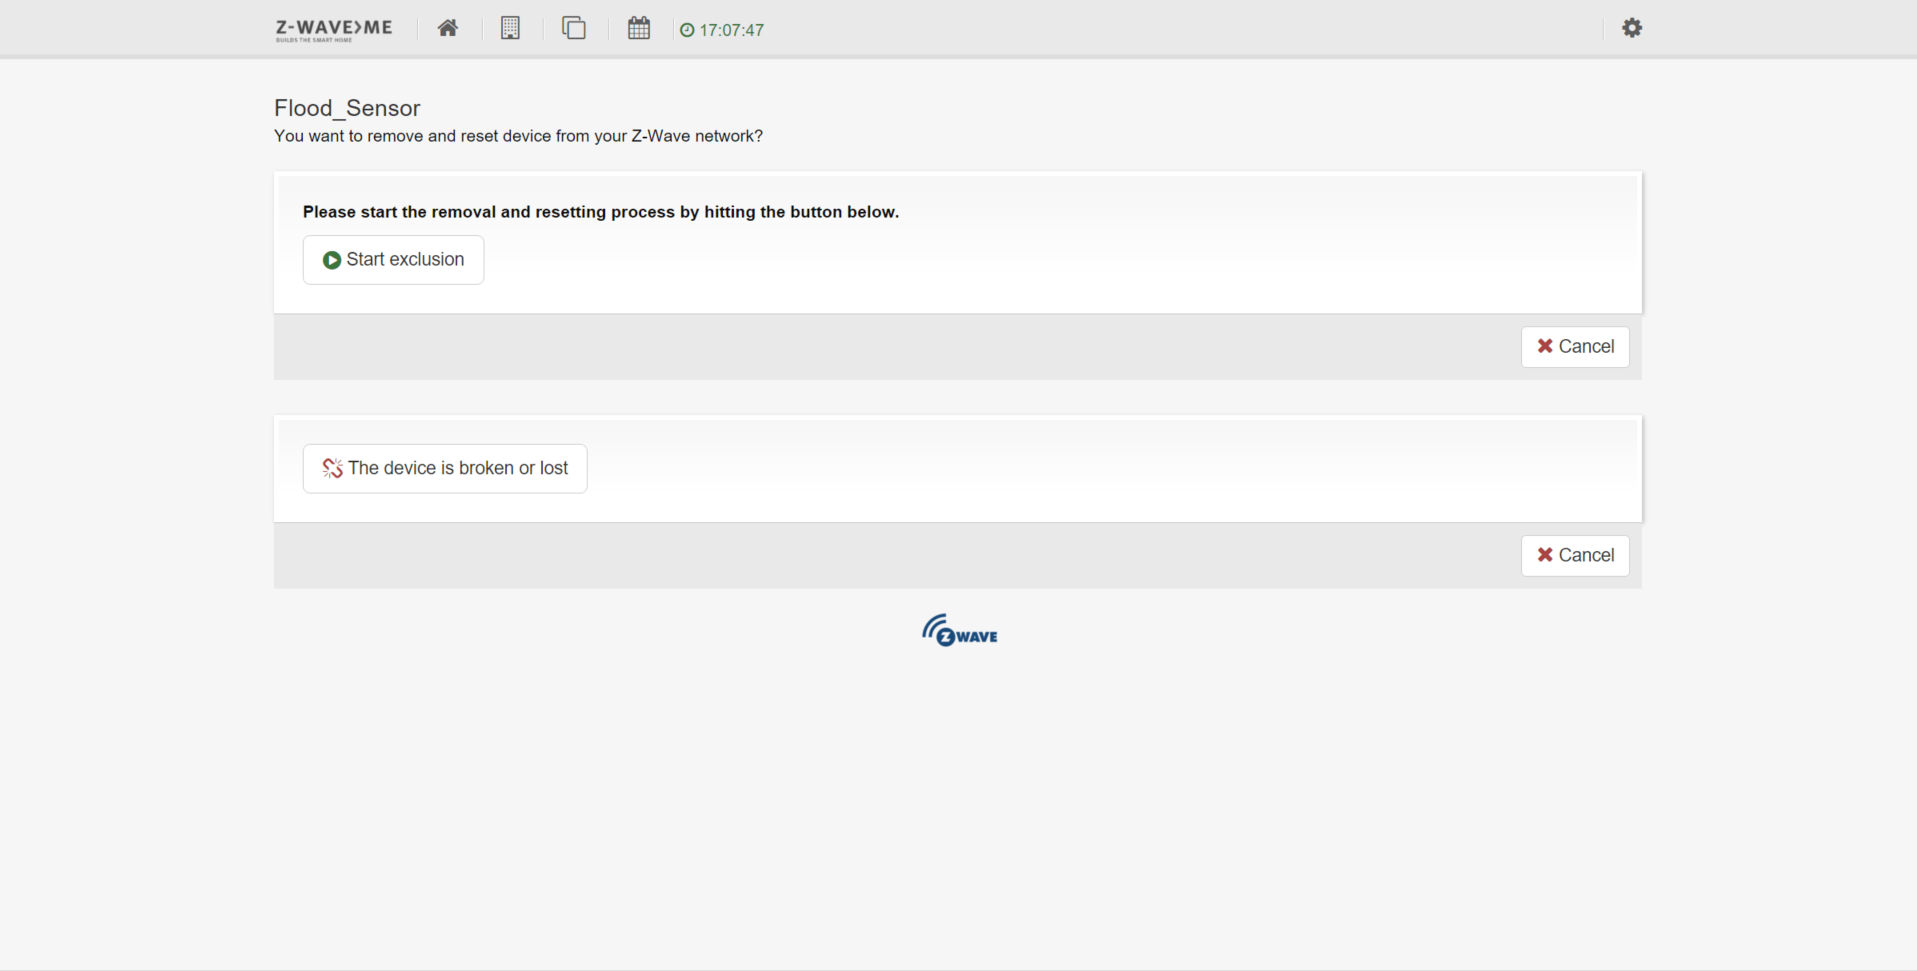
\includegraphics[scale=0.5]{./latex/Images/png/delete_zwaveme.png}\newline

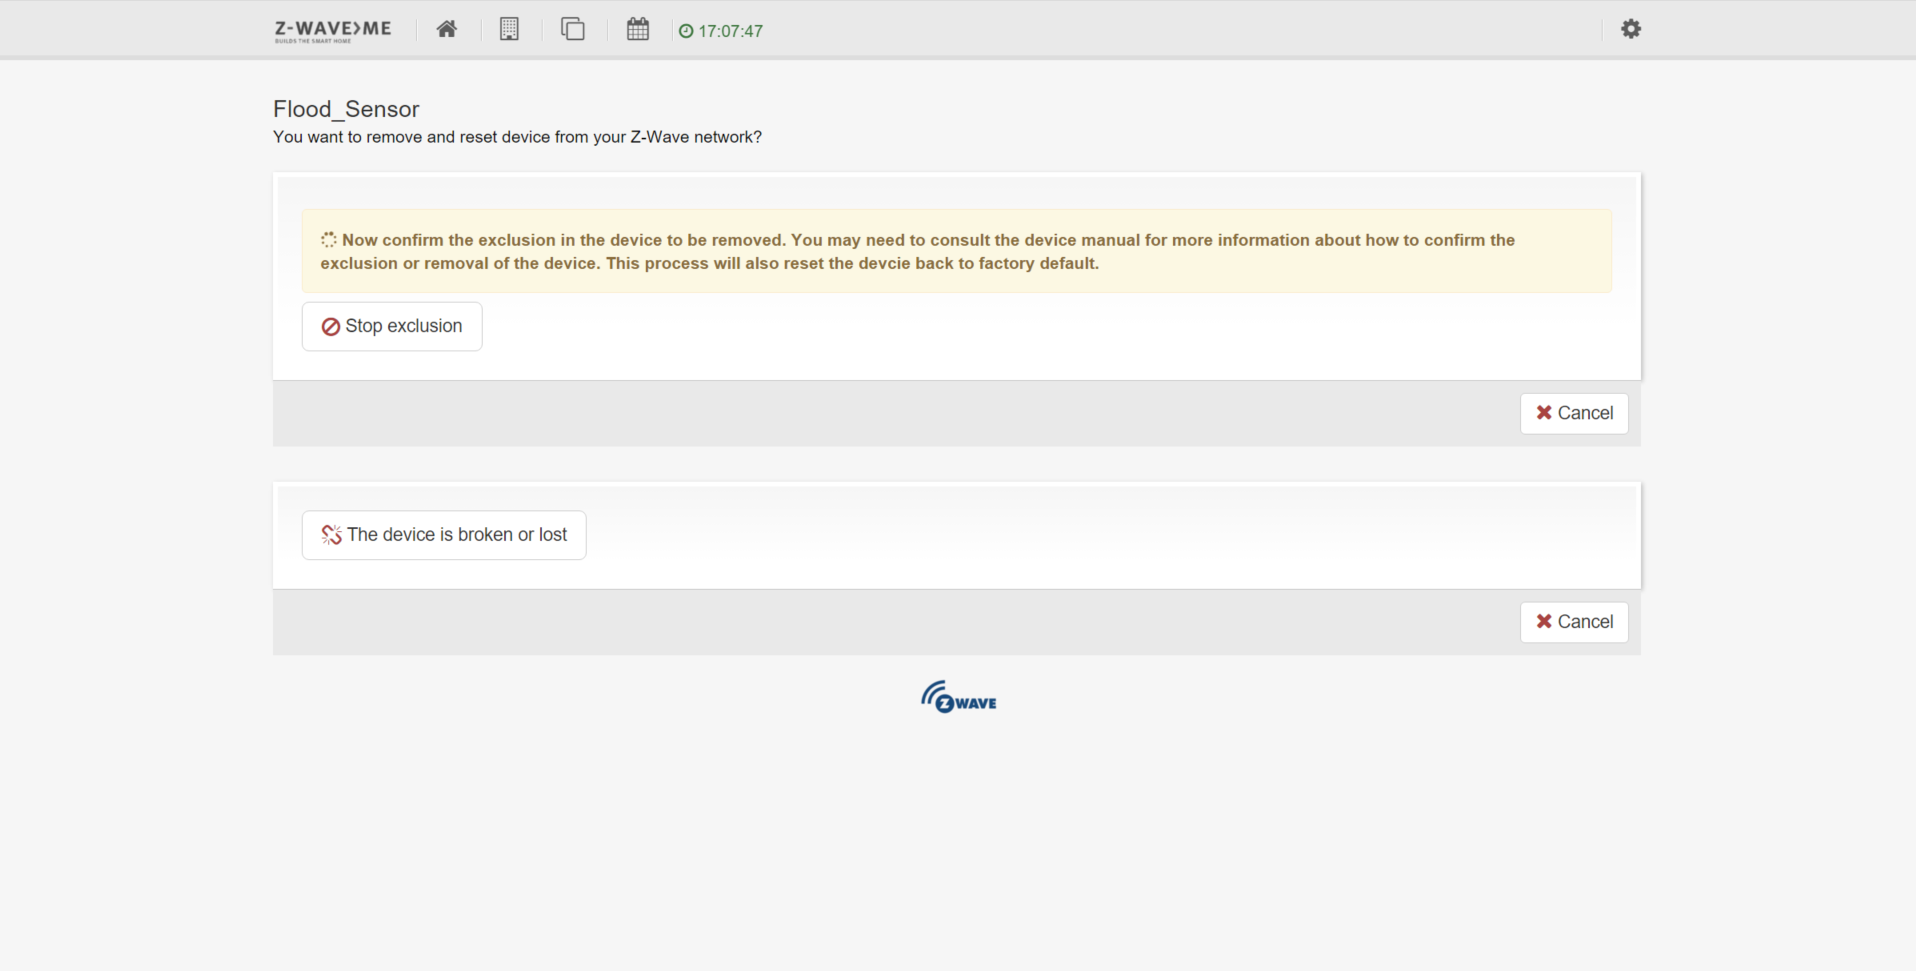
\includegraphics[scale=0.5]{./latex/Images/png/exclusion_zwaveme.png}\newline

--> Le device sera alors exclu


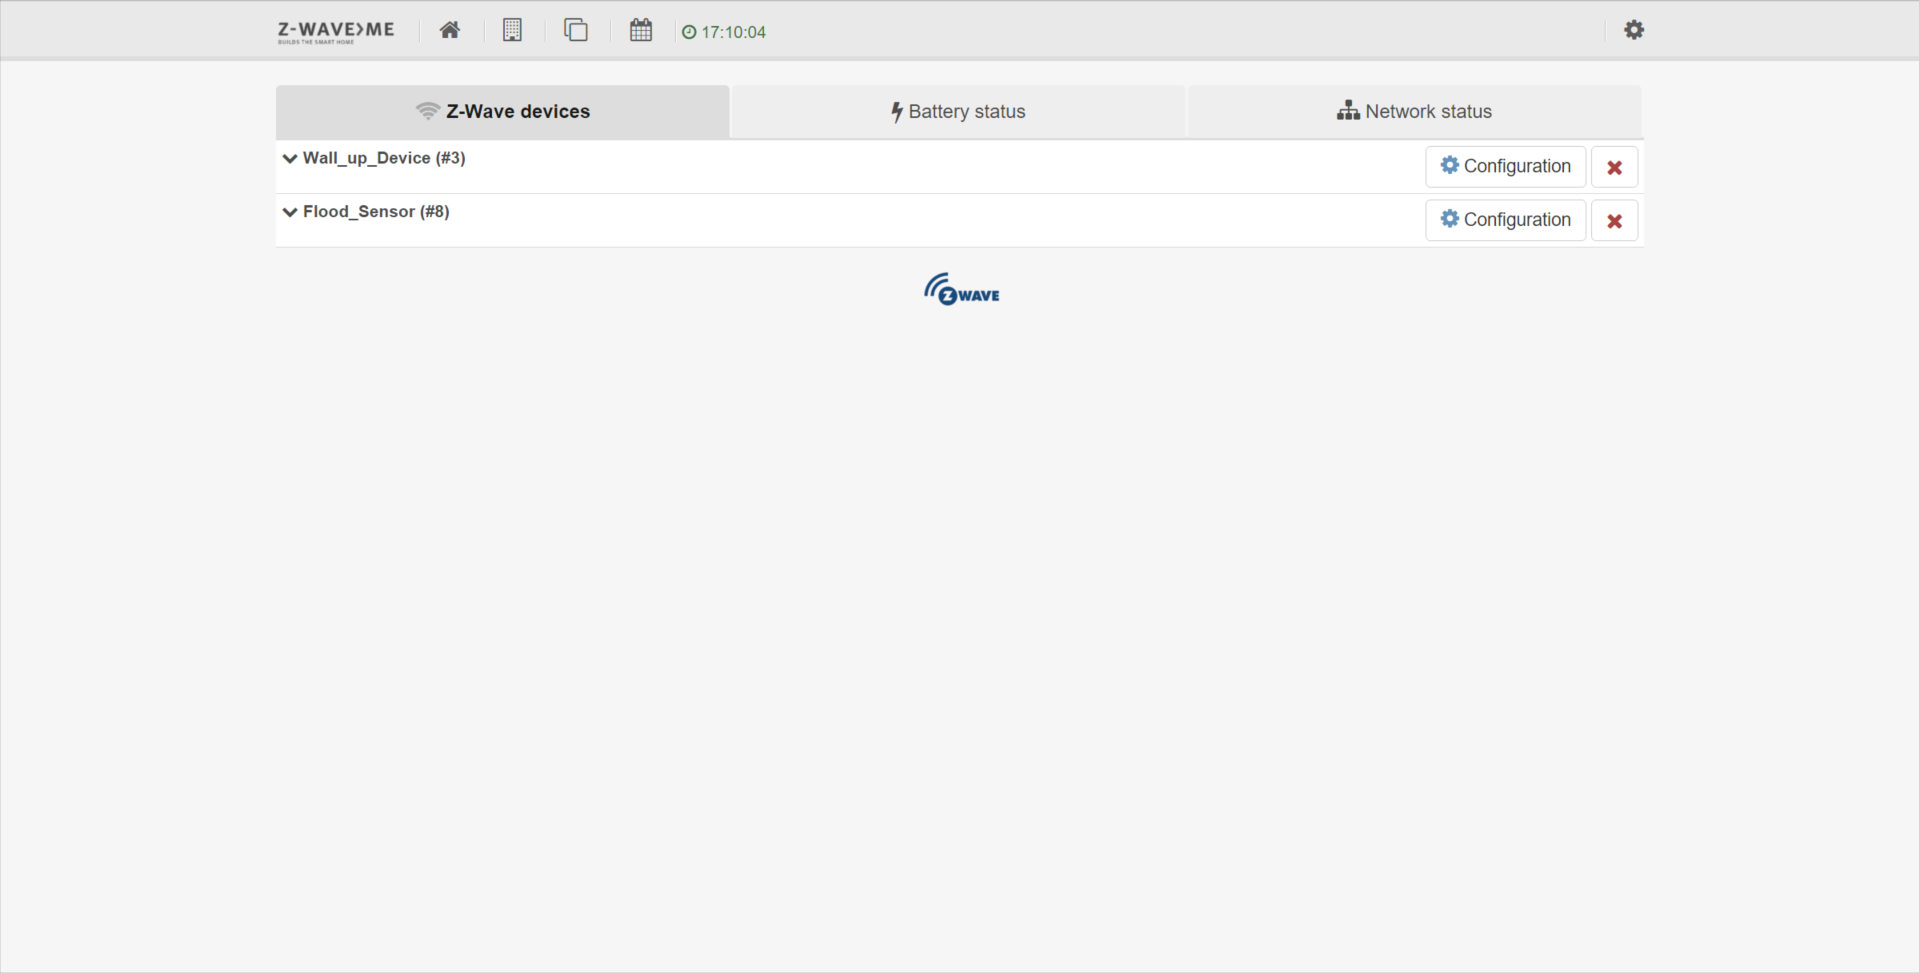
\includegraphics[scale=0.5]{./latex/Images/png/devices_exclu_zwaveme.png}\newline


* Les applications disponibles concernants les capteurs:

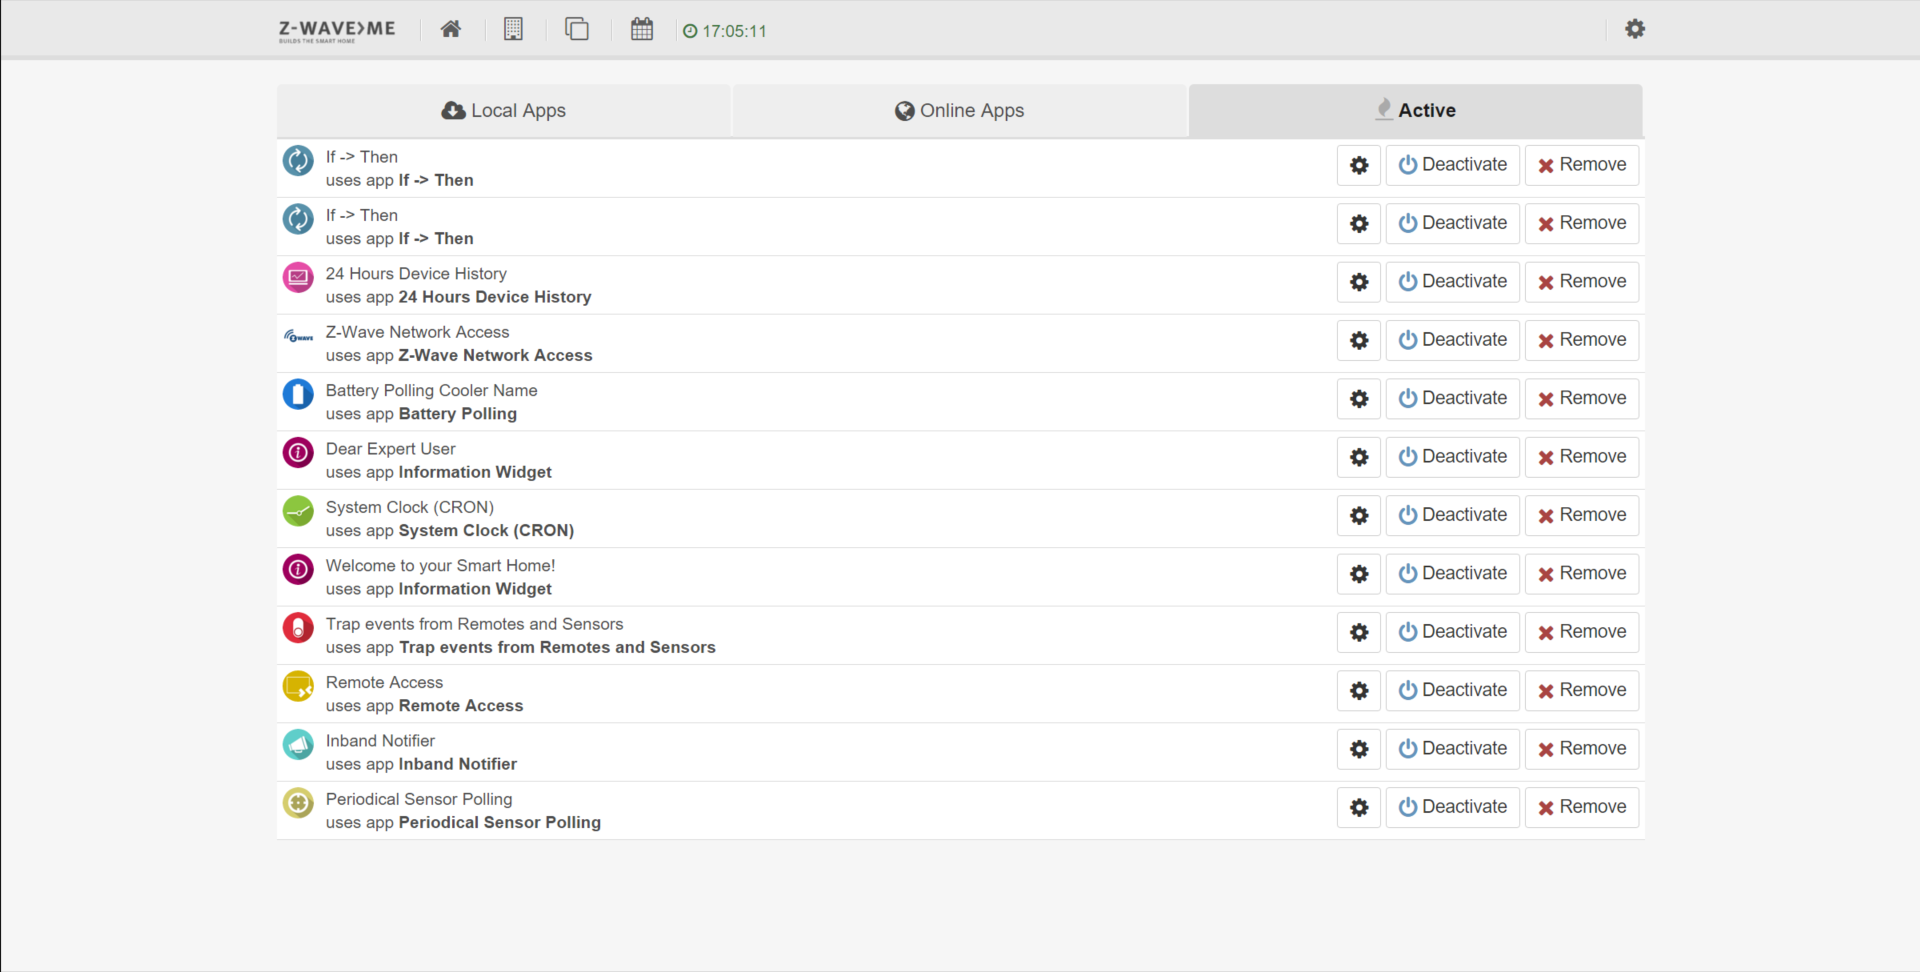
\includegraphics[scale=0.5]{./latex/Images/png/app_zwaveme.png}\newline 

* Dans le mode expert, vous pouvez remarquer l'état de vos capteurs

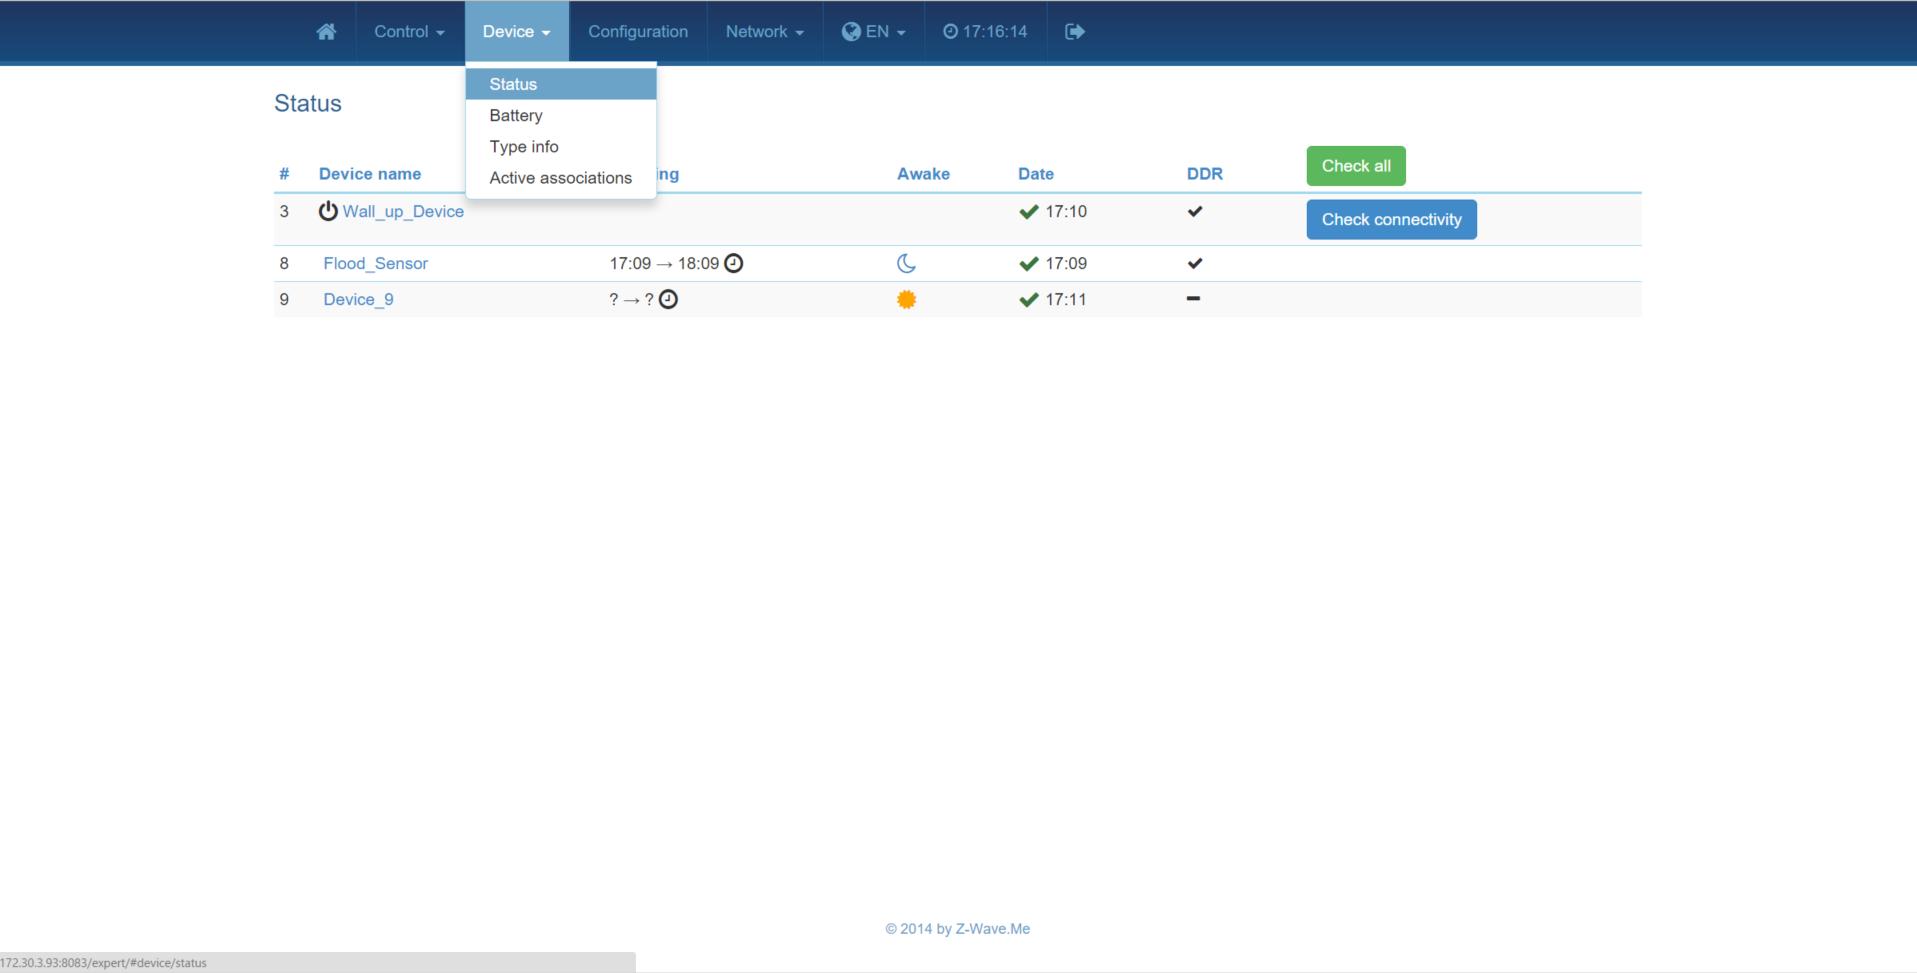
\includegraphics[scale=0.5]{./latex/Images/png/device_Status.png}\newline


* Une description détaillée des capteurs disponibles (mode expert)

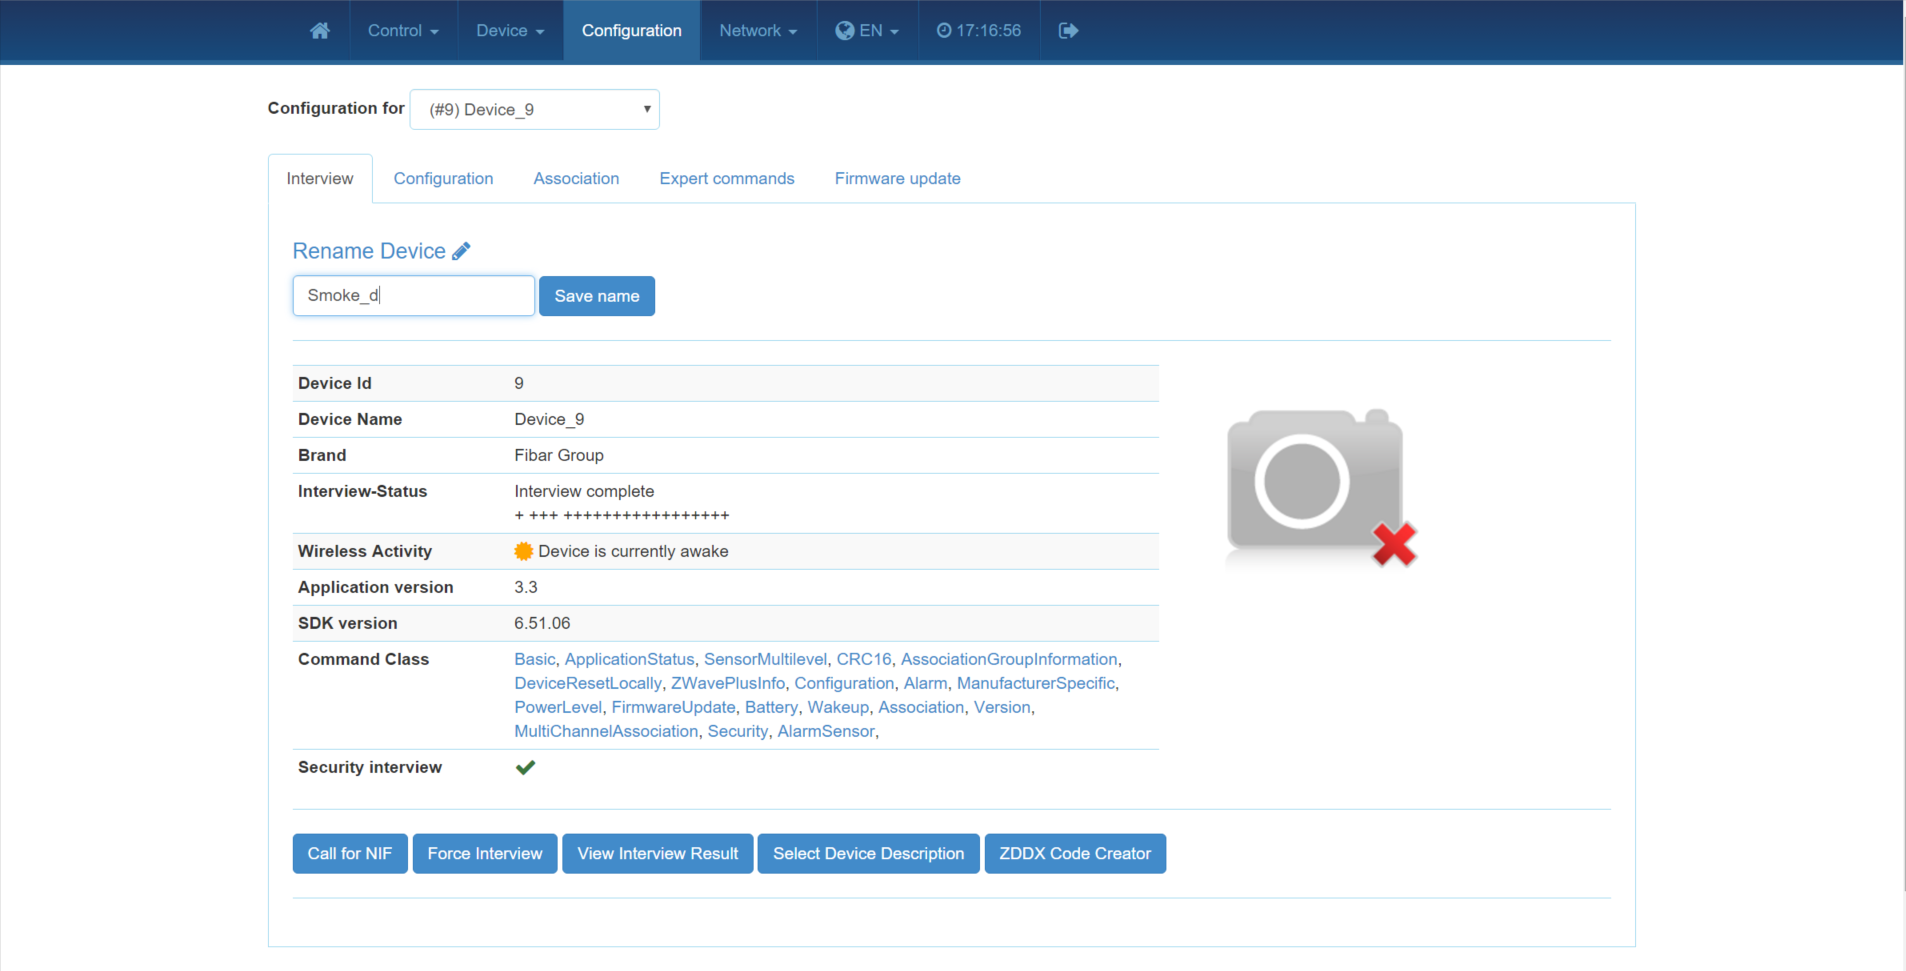
\includegraphics[scale=0.5]{./latex/Images/png/description_zwaveme.png}\newline

* Le log des capteurs qui permet de vérifier l'état des capteurs en temps continu et réel (Veille, On, Off, ...)


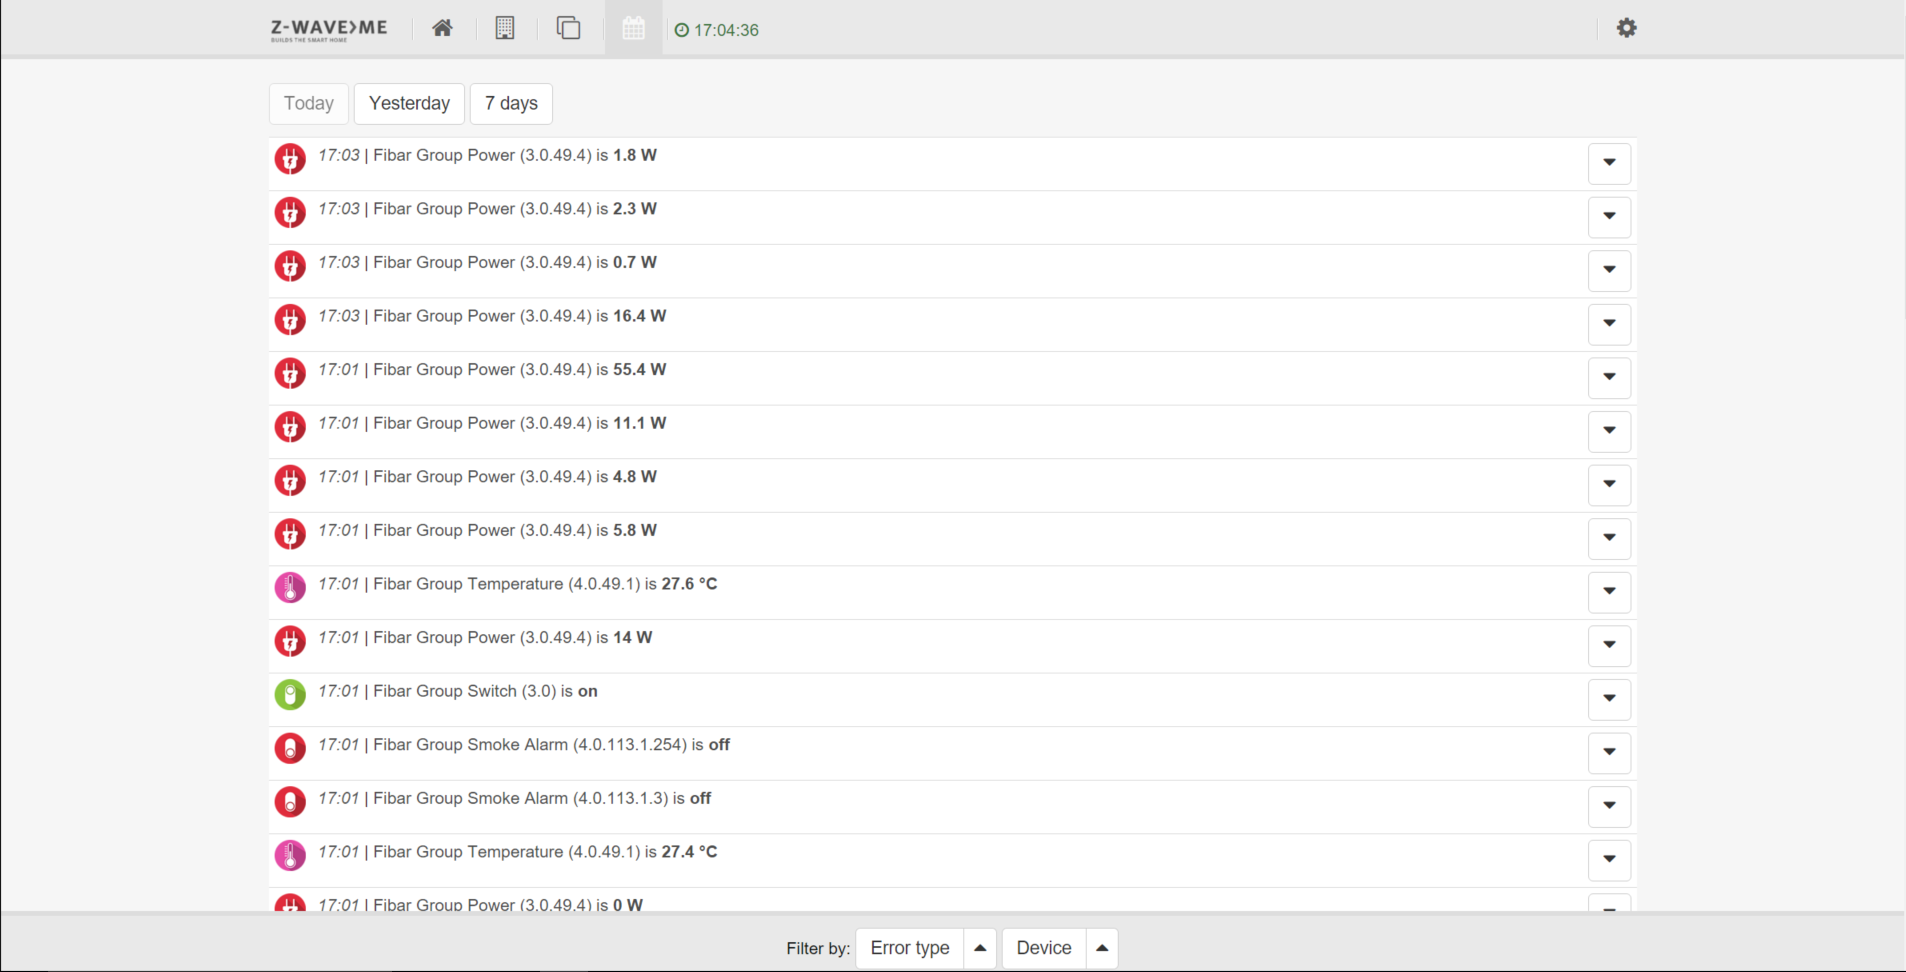
\includegraphics[scale=0.5]{./latex/Images/png/log_zwaveme.png}\newline

* Ajouter des chambres ou des homes ( Notre application Android se base sur ce principe)

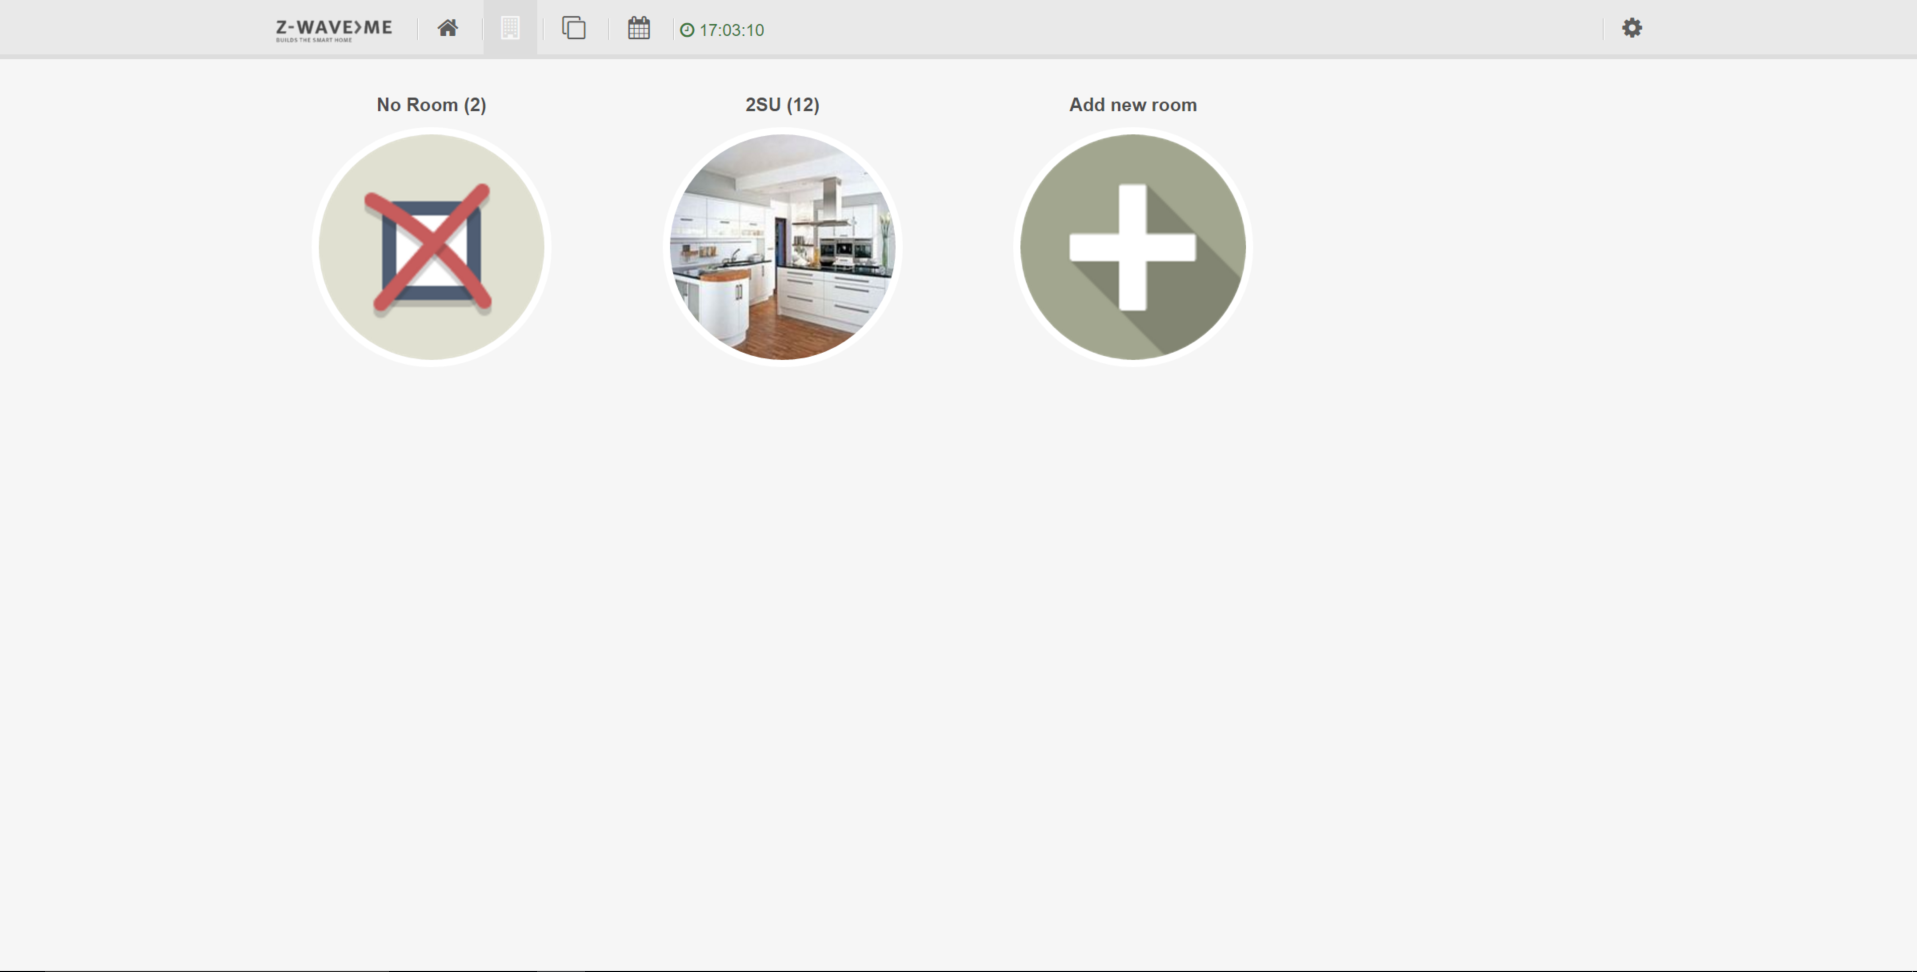
\includegraphics[scale=0.5]{./latex/Images/png/room_zwaveme.png}\newline

* Desciption des capteurs (mode expert)

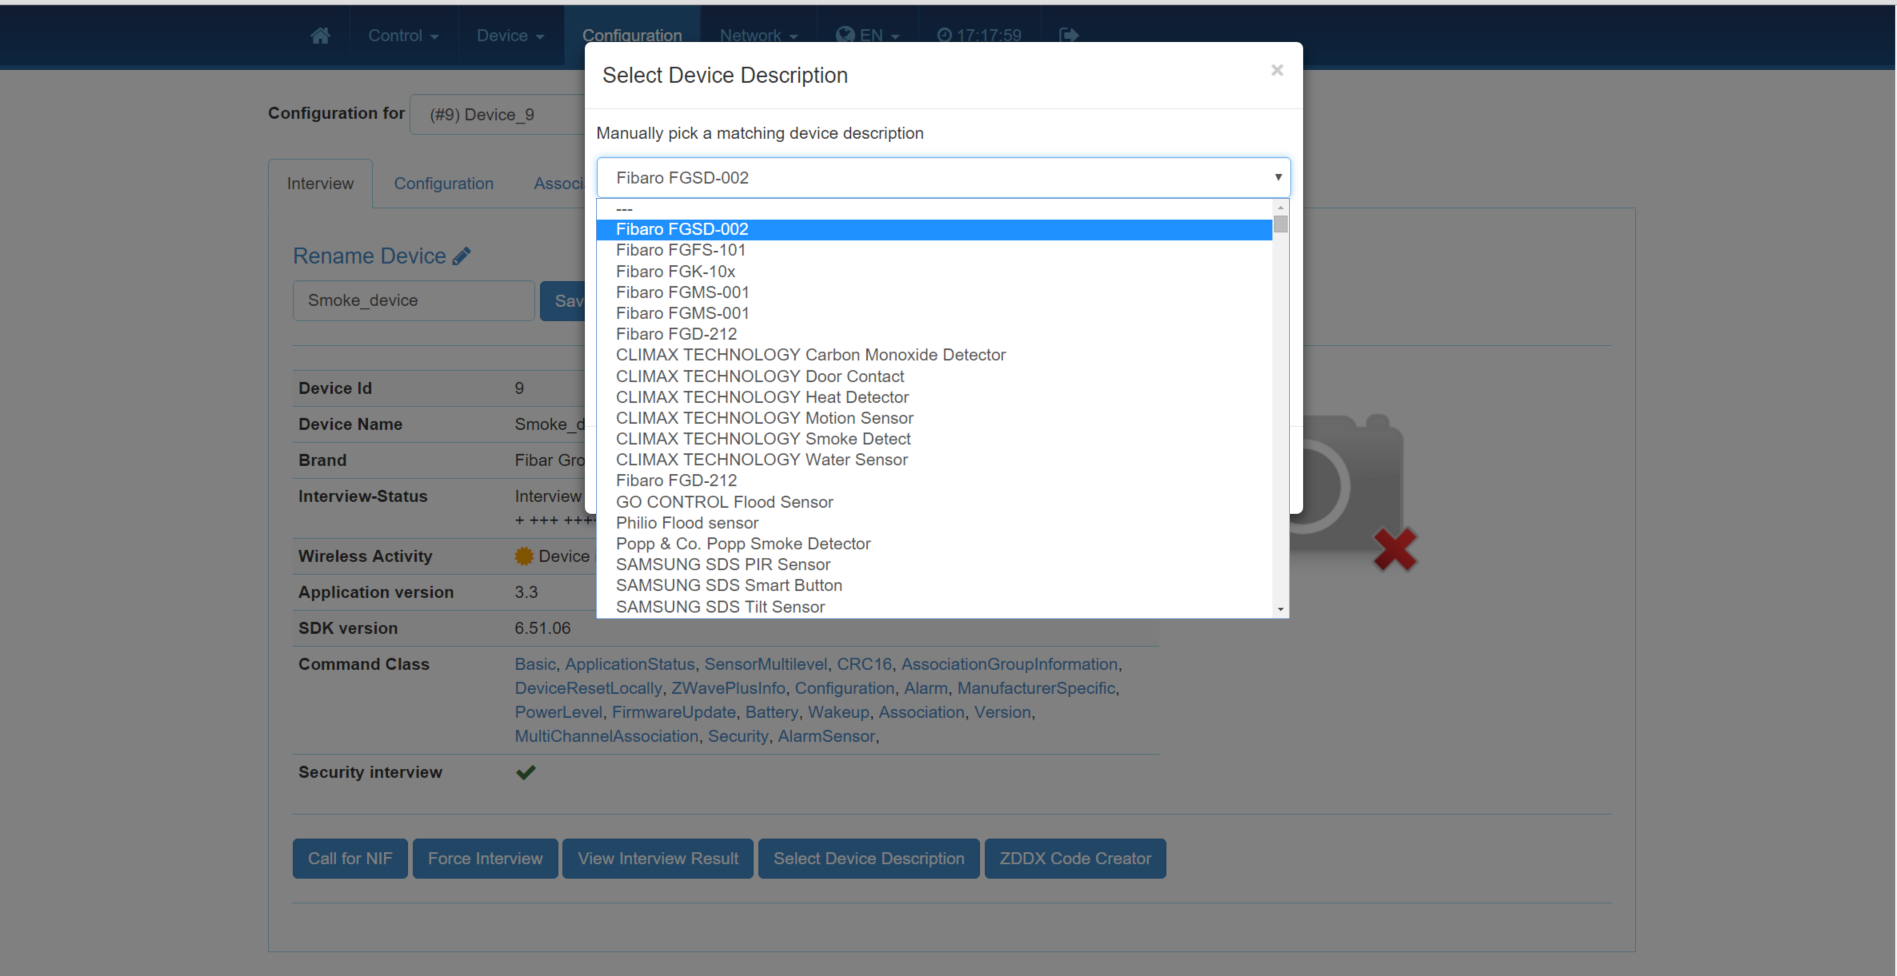
\includegraphics[scale=0.5]{./latex/Images/png/smoke_description_zwaveme.png}\newline

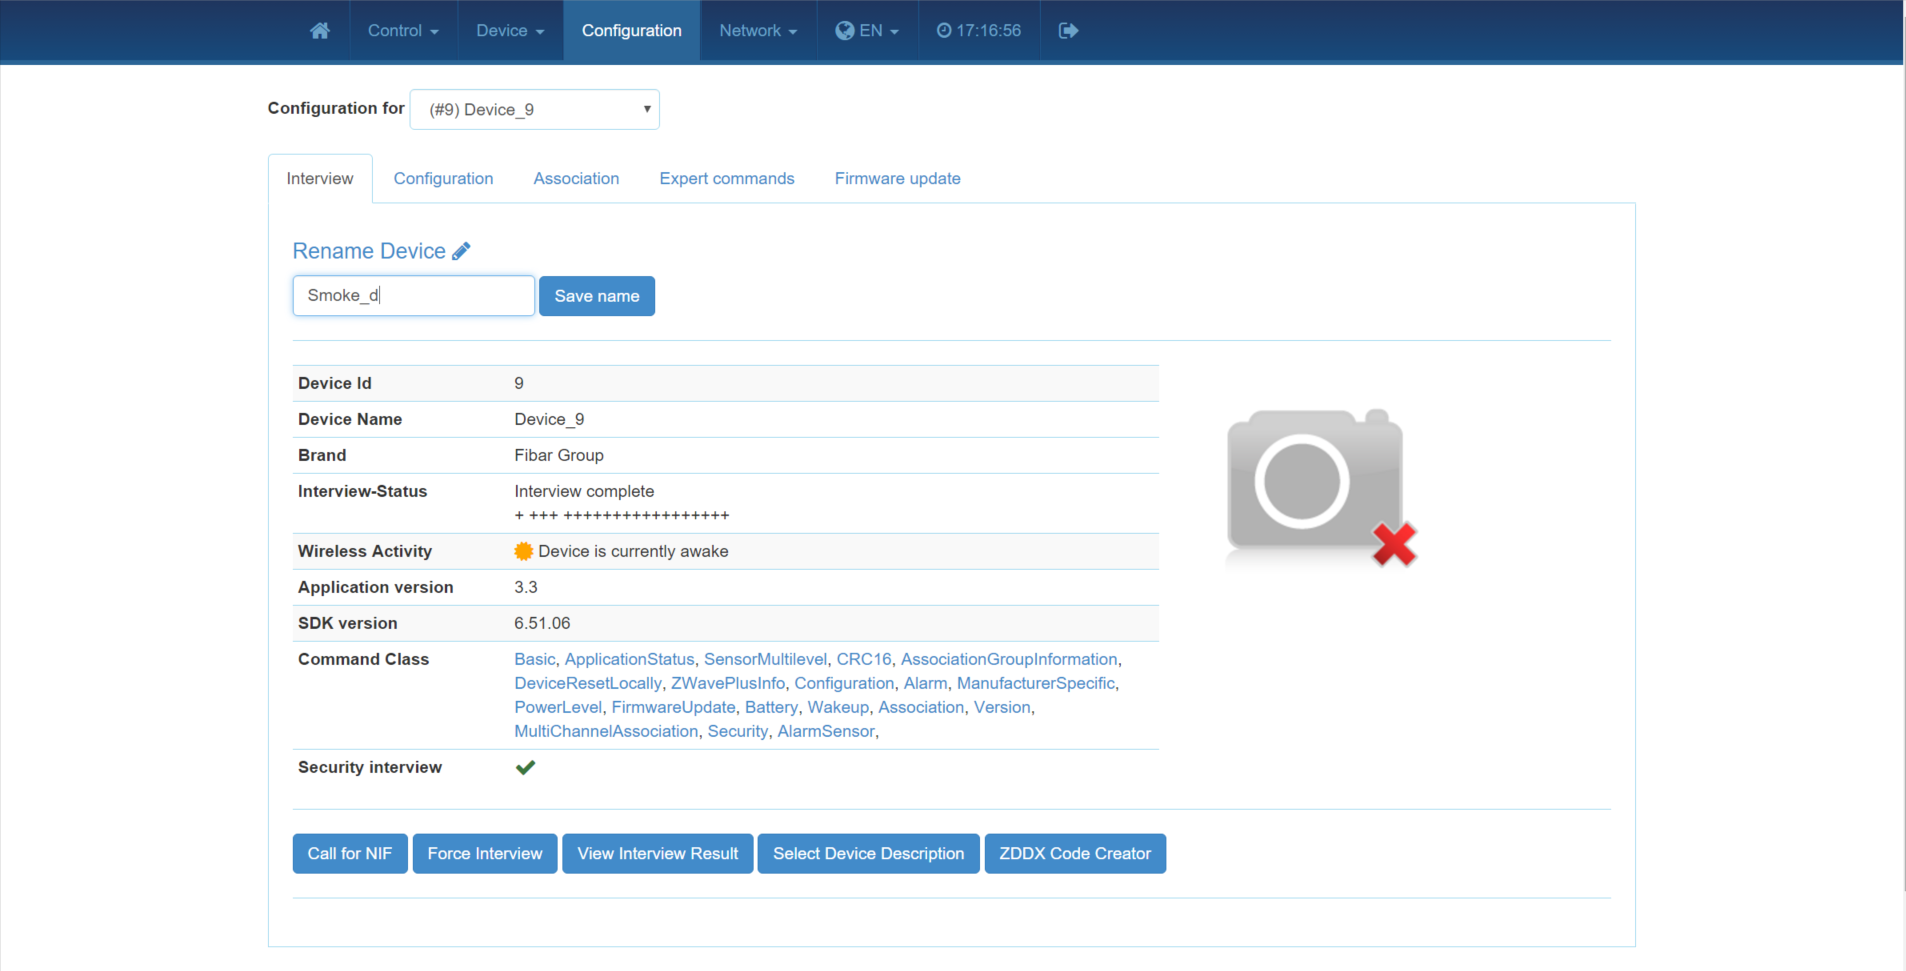
\includegraphics[scale=0.5]{./latex/Images/png/description_zwaveme.png}\newline

* Une vidéo d'une de nos démonstration sur le flood sensor se trouve sur ce lien:
 \href{https://www.youtube.com/watch?v=nNWe8rKhf1o&feature=youtu.be}

\end{document}
